\documentclass{article}
\usepackage[a4paper,left=3cm,right=3cm,top=3cm,bottom=3cm]{geometry}
\usepackage[utf8]{inputenc}
\usepackage[T1]{fontenc}
\usepackage{latexsym,amsfonts,amsmath,amssymb,amstext,graphicx,titlesec,ae,aecompl,mathtools,tabularx, multirow, cancel, nicefrac,subcaption, blindtext, floatrow}
\setlength{\parindent}{0pt}
\newfloatcommand{capbtabbox}{table}[][\FBwidth]


\begin{document}

\begin{titlepage}
       \begin{center}
             \begin{huge}
				   %% Update assignment number here
                   \textbf{Assignment 4}
             \end{huge}
       \end{center}

       \begin{center}
             \begin{large}
                   Computational Intelligence, SS2020
             \end{large}
       \end{center}

       \begin{center}
 \begin{tabularx}{\textwidth}{|>{\hsize=.33\hsize}X|>{\hsize=.33\hsize}X|>{\hsize=.33\hsize}X|} 

                   \hline
                   \multicolumn{3}{|c|}{\textbf{Team Members}} \\
                   \hline
                   Last name & First name & Matriculation Number \\
                   \hline
                   Blöcher & Christian & 01573246 \\
                   \hline
                   Bürgener & Max & 01531577 \\
                   \hline
                    &  &  \\
                   \hline

             \end{tabularx}
       \end{center}
\end{titlepage}


\section{Linear SVM}

\subsection{Plots}

\begin{figure}[!ht]
\centering
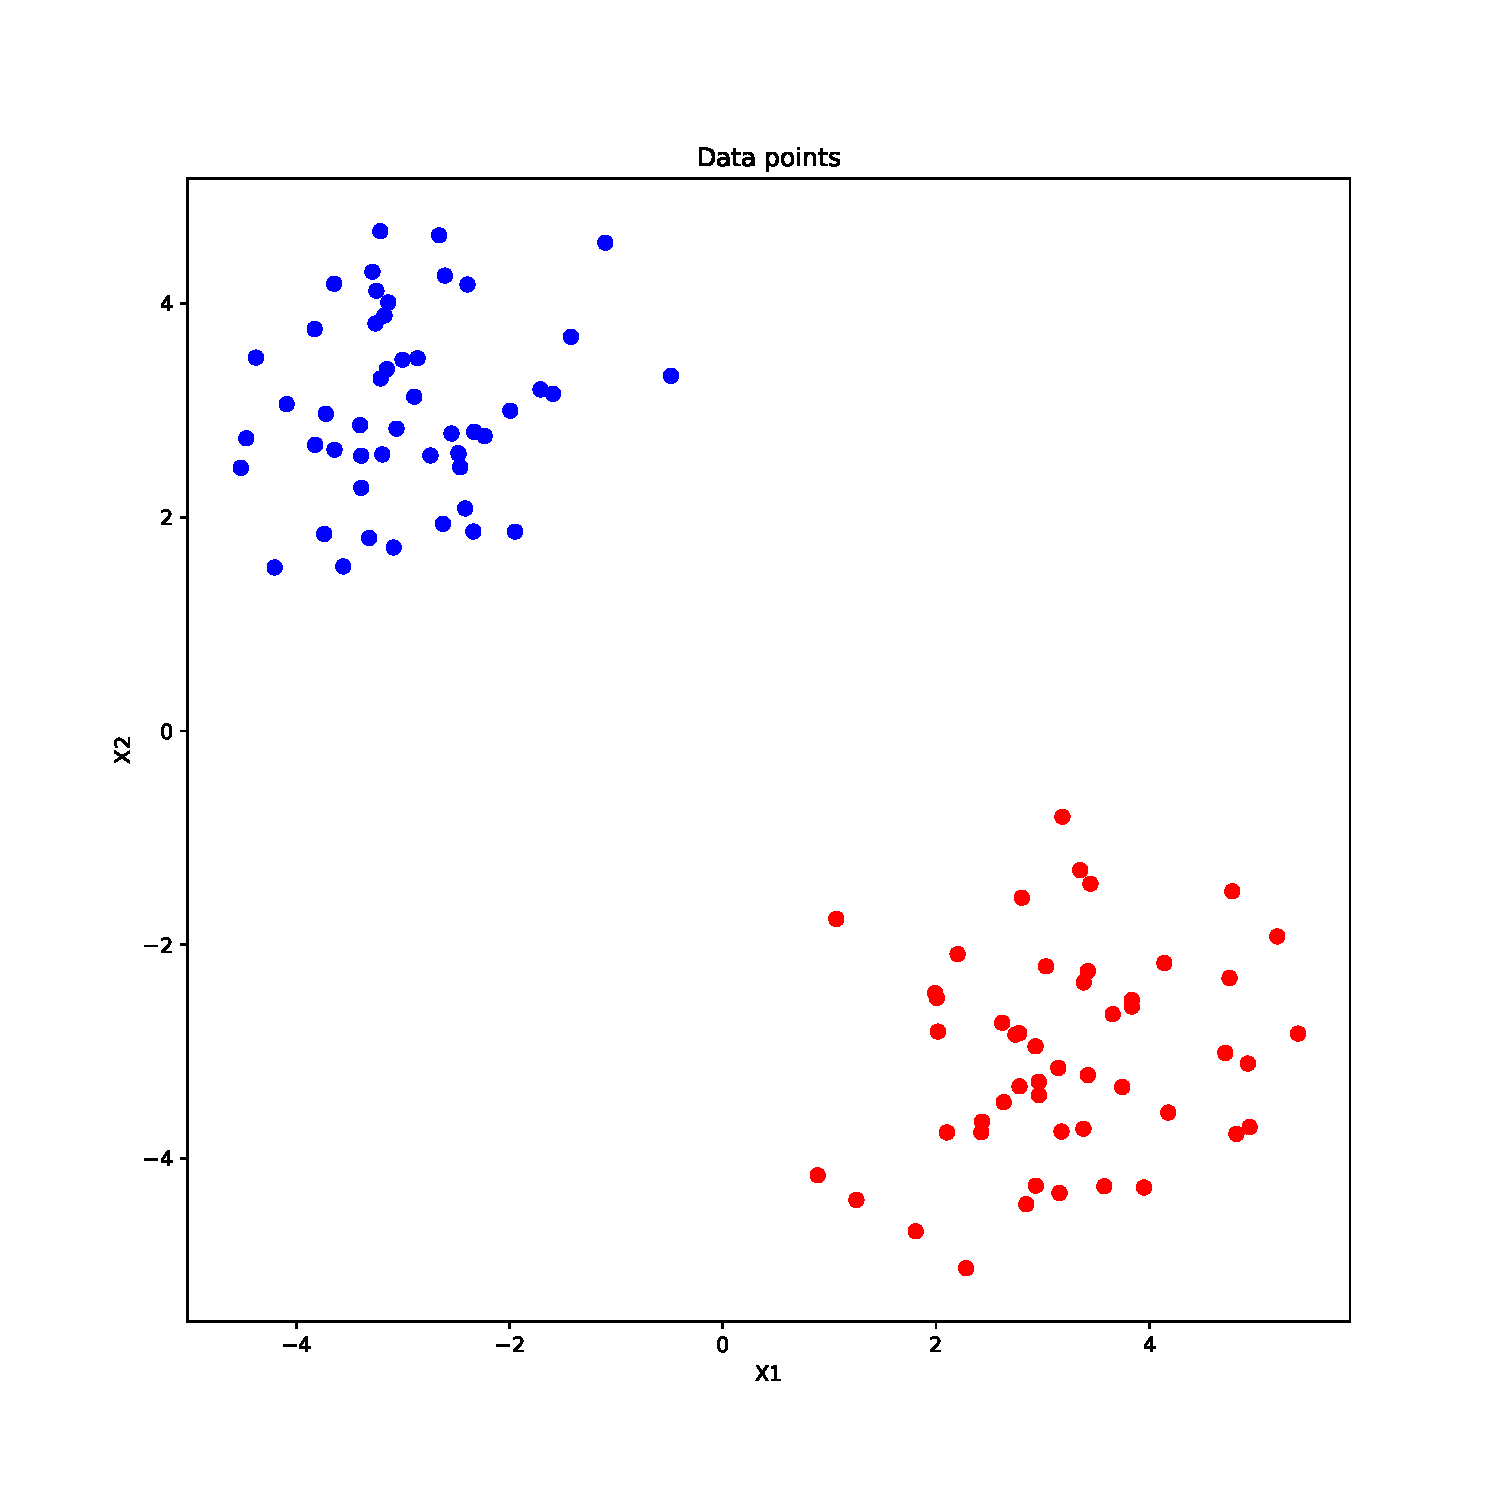
\includegraphics[width=.6\textwidth]{./Figures/1_data}
\caption{Dataset}
\label{Dataset}
\end{figure}

\begin{figure}[!ht]
	\makebox[\textwidth]{
	\begin{subfigure}{0.6\textwidth}
	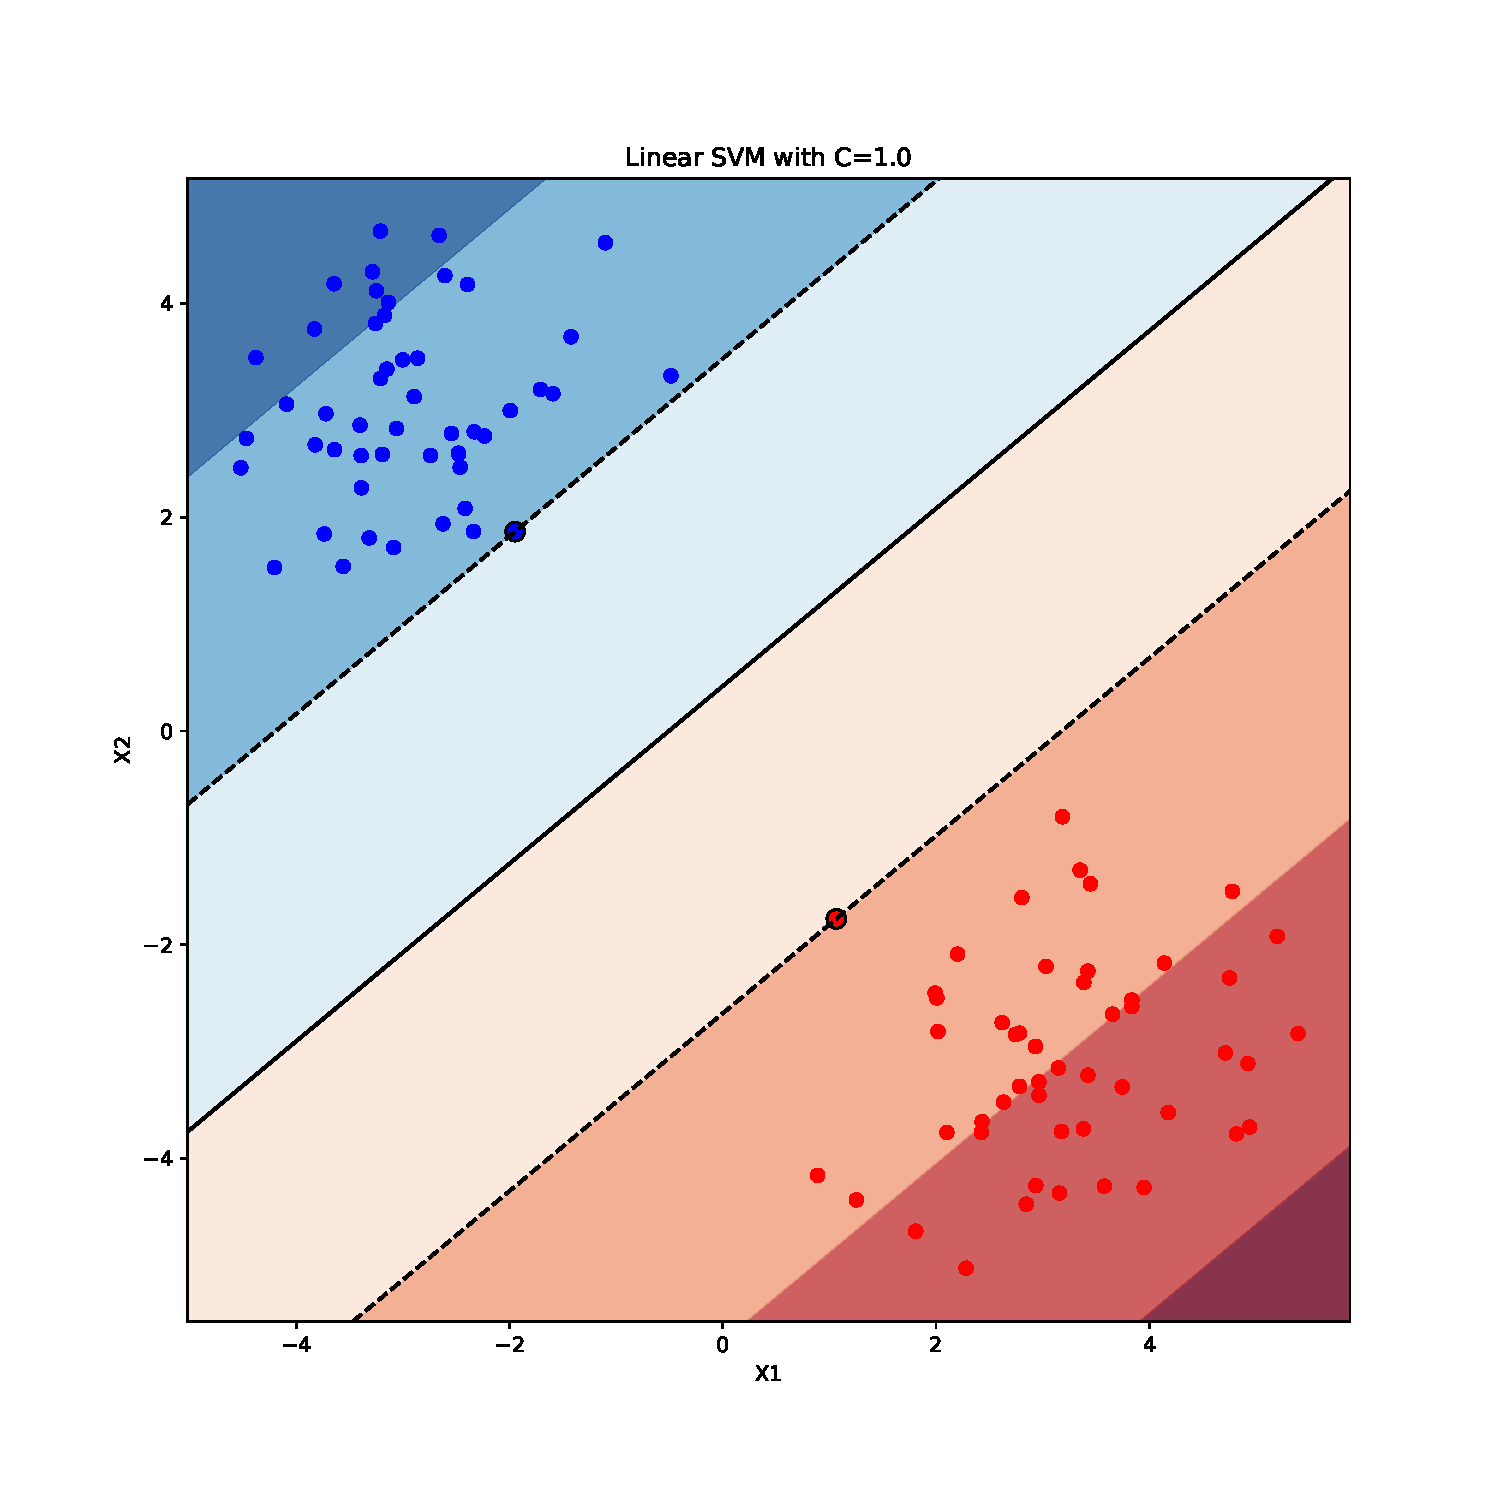
\includegraphics[width=\textwidth]{./Figures/1a_bound.pdf}
	\caption{Dataset}
	\end{subfigure}
	\begin{subfigure}{0.6\textwidth}
	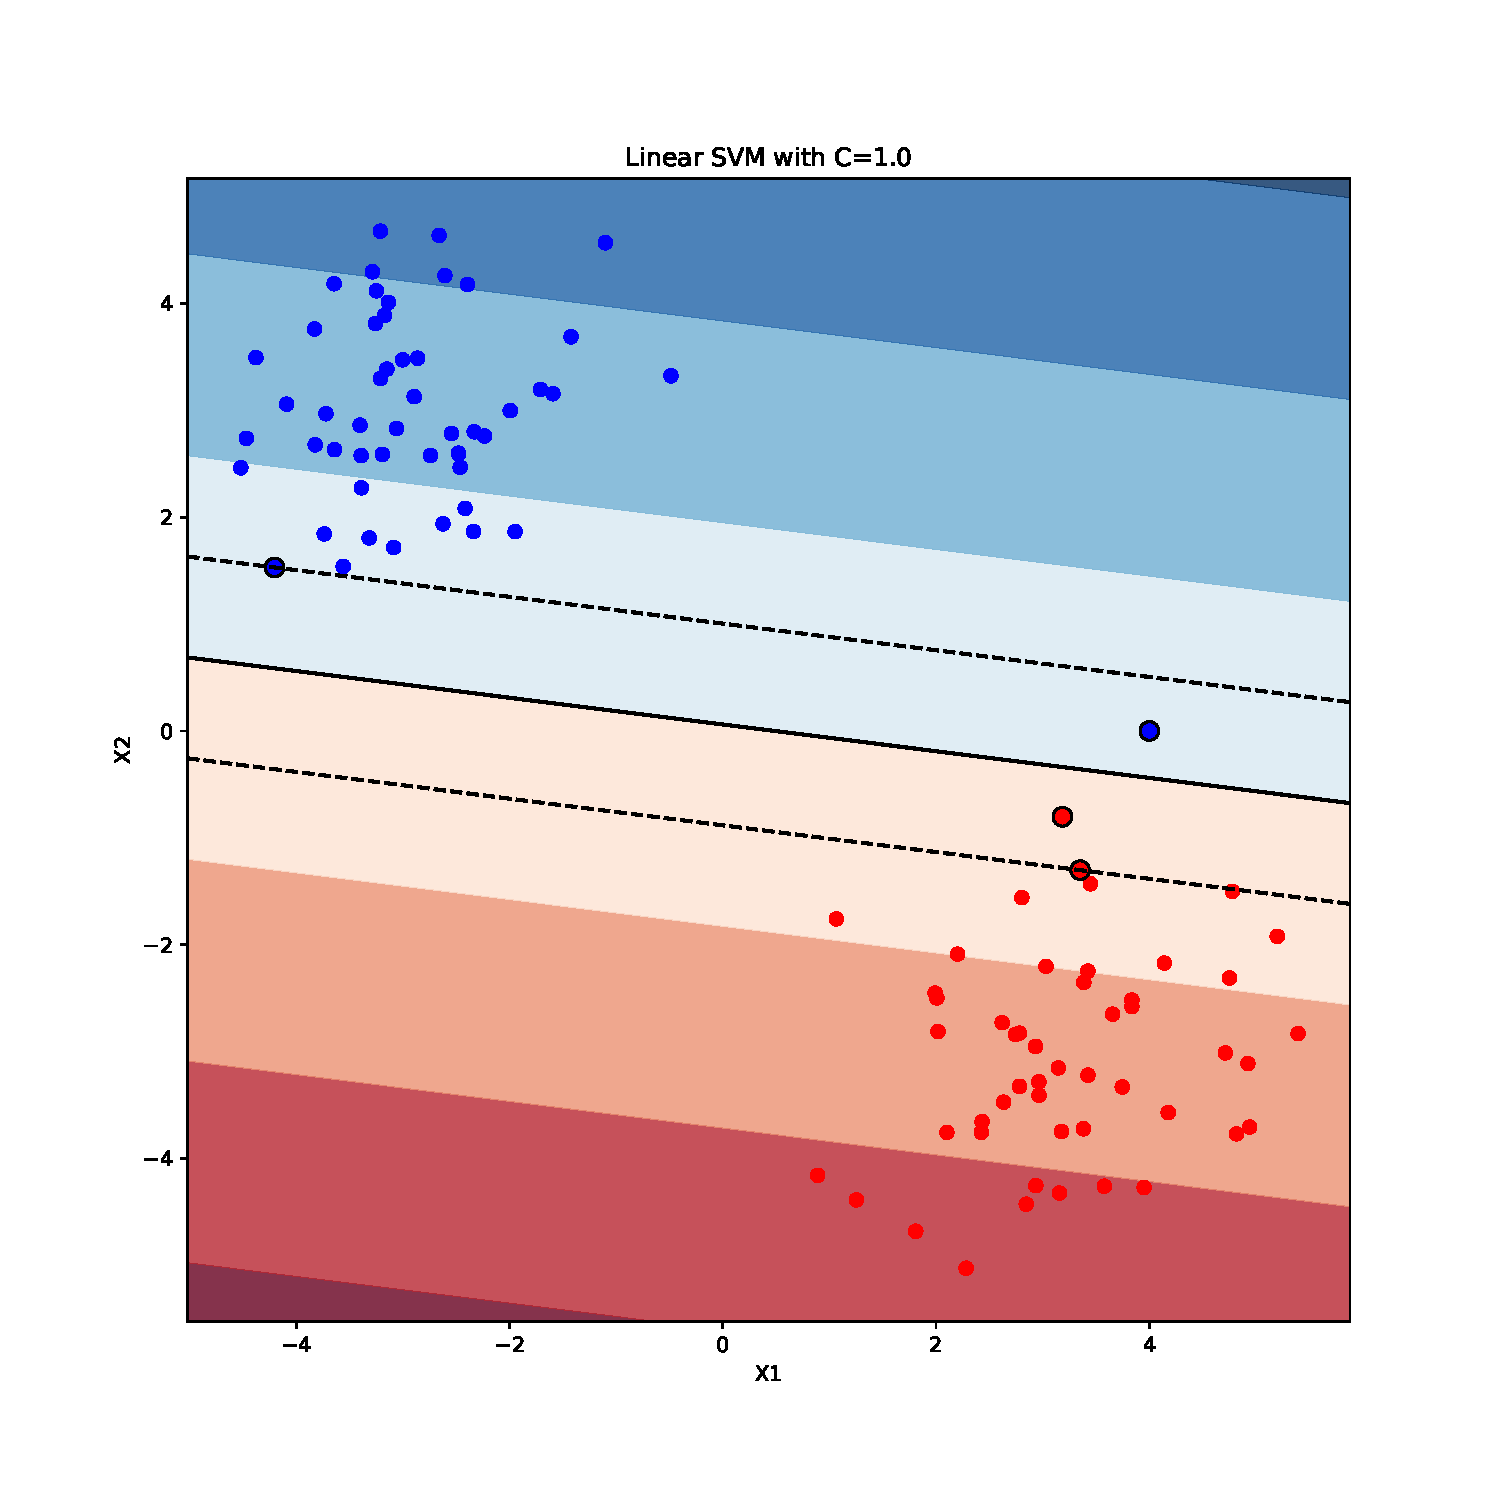
\includegraphics[width=\textwidth]{./Figures/1b_bound}
	\caption{Dataset with additional data point}
	\end{subfigure}
	}	
	\caption{Classification of the dataset using SVM}
	\label{SVM_classification}
\end{figure}

\begin{figure}[!ht]
    \centering
    \makebox[\textwidth]{
    \begin{subfigure}{0.6\textwidth}
    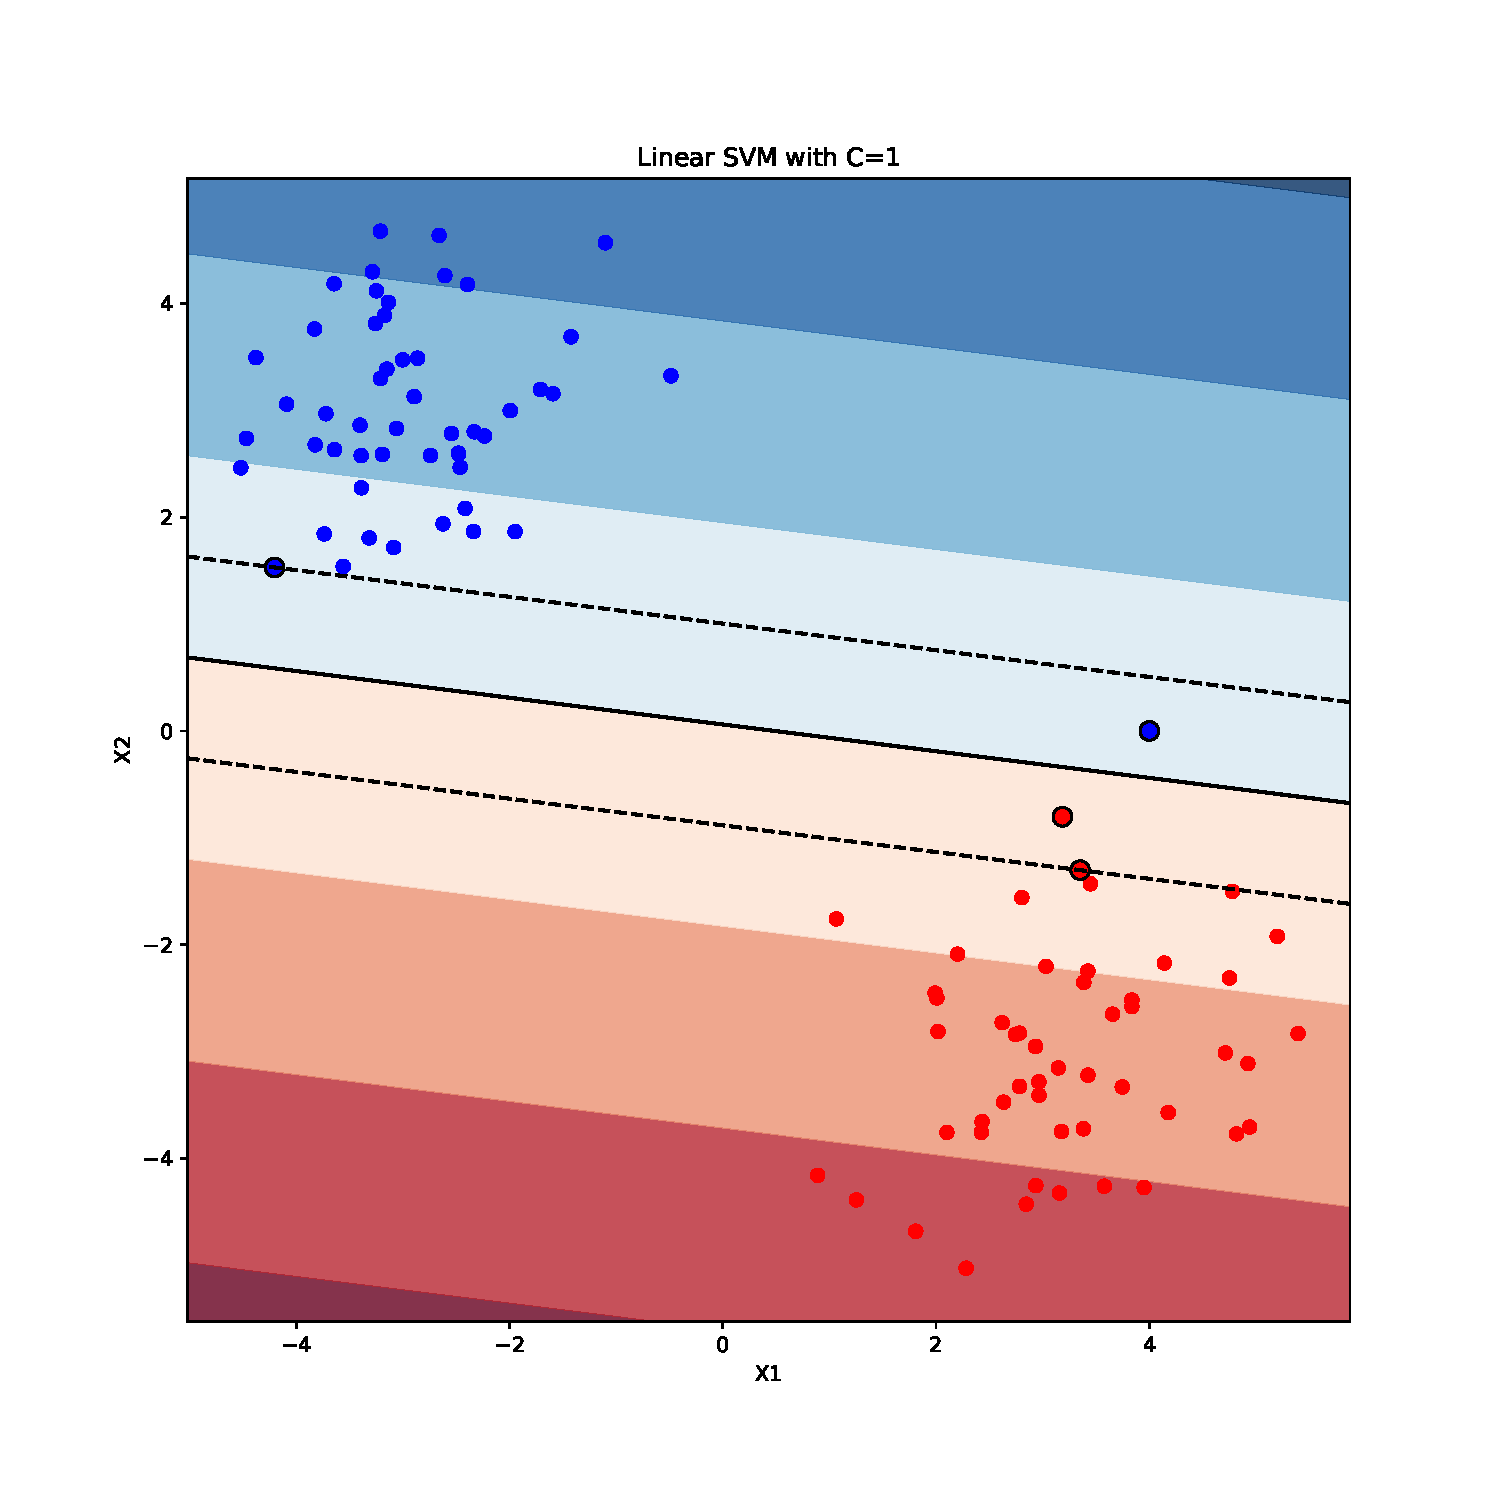
\includegraphics[width=\textwidth]{./Figures/1c_bound_C1.pdf}
    \caption{$C=1$}
    \end{subfigure}
    \begin{subfigure}{0.6\textwidth}
    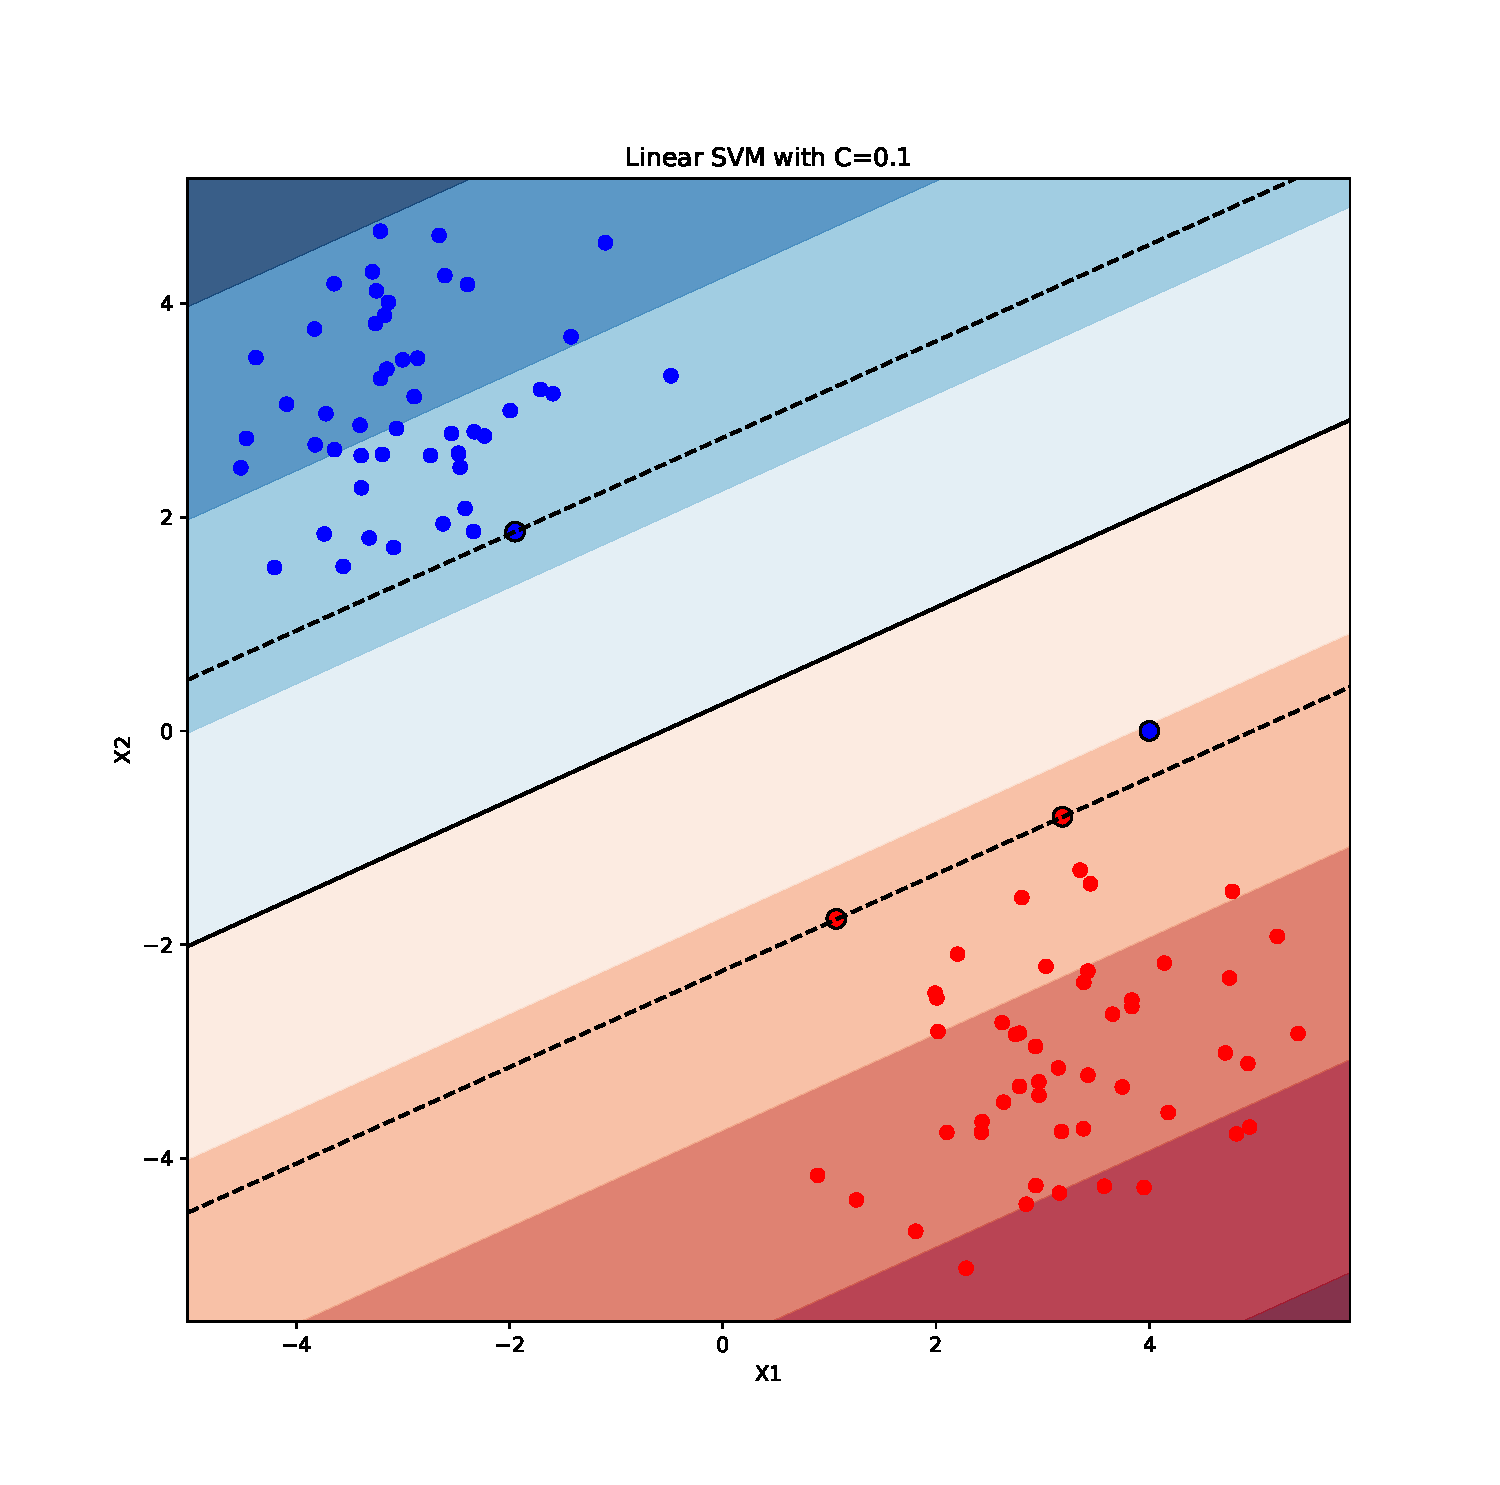
\includegraphics[width=\textwidth]{./Figures/1c_bound_C01.pdf}
    \caption{$C=0,1$}
    \end{subfigure}
    }
    
    \makebox[\textwidth]{
    \begin{subfigure}{0.6\textwidth}
    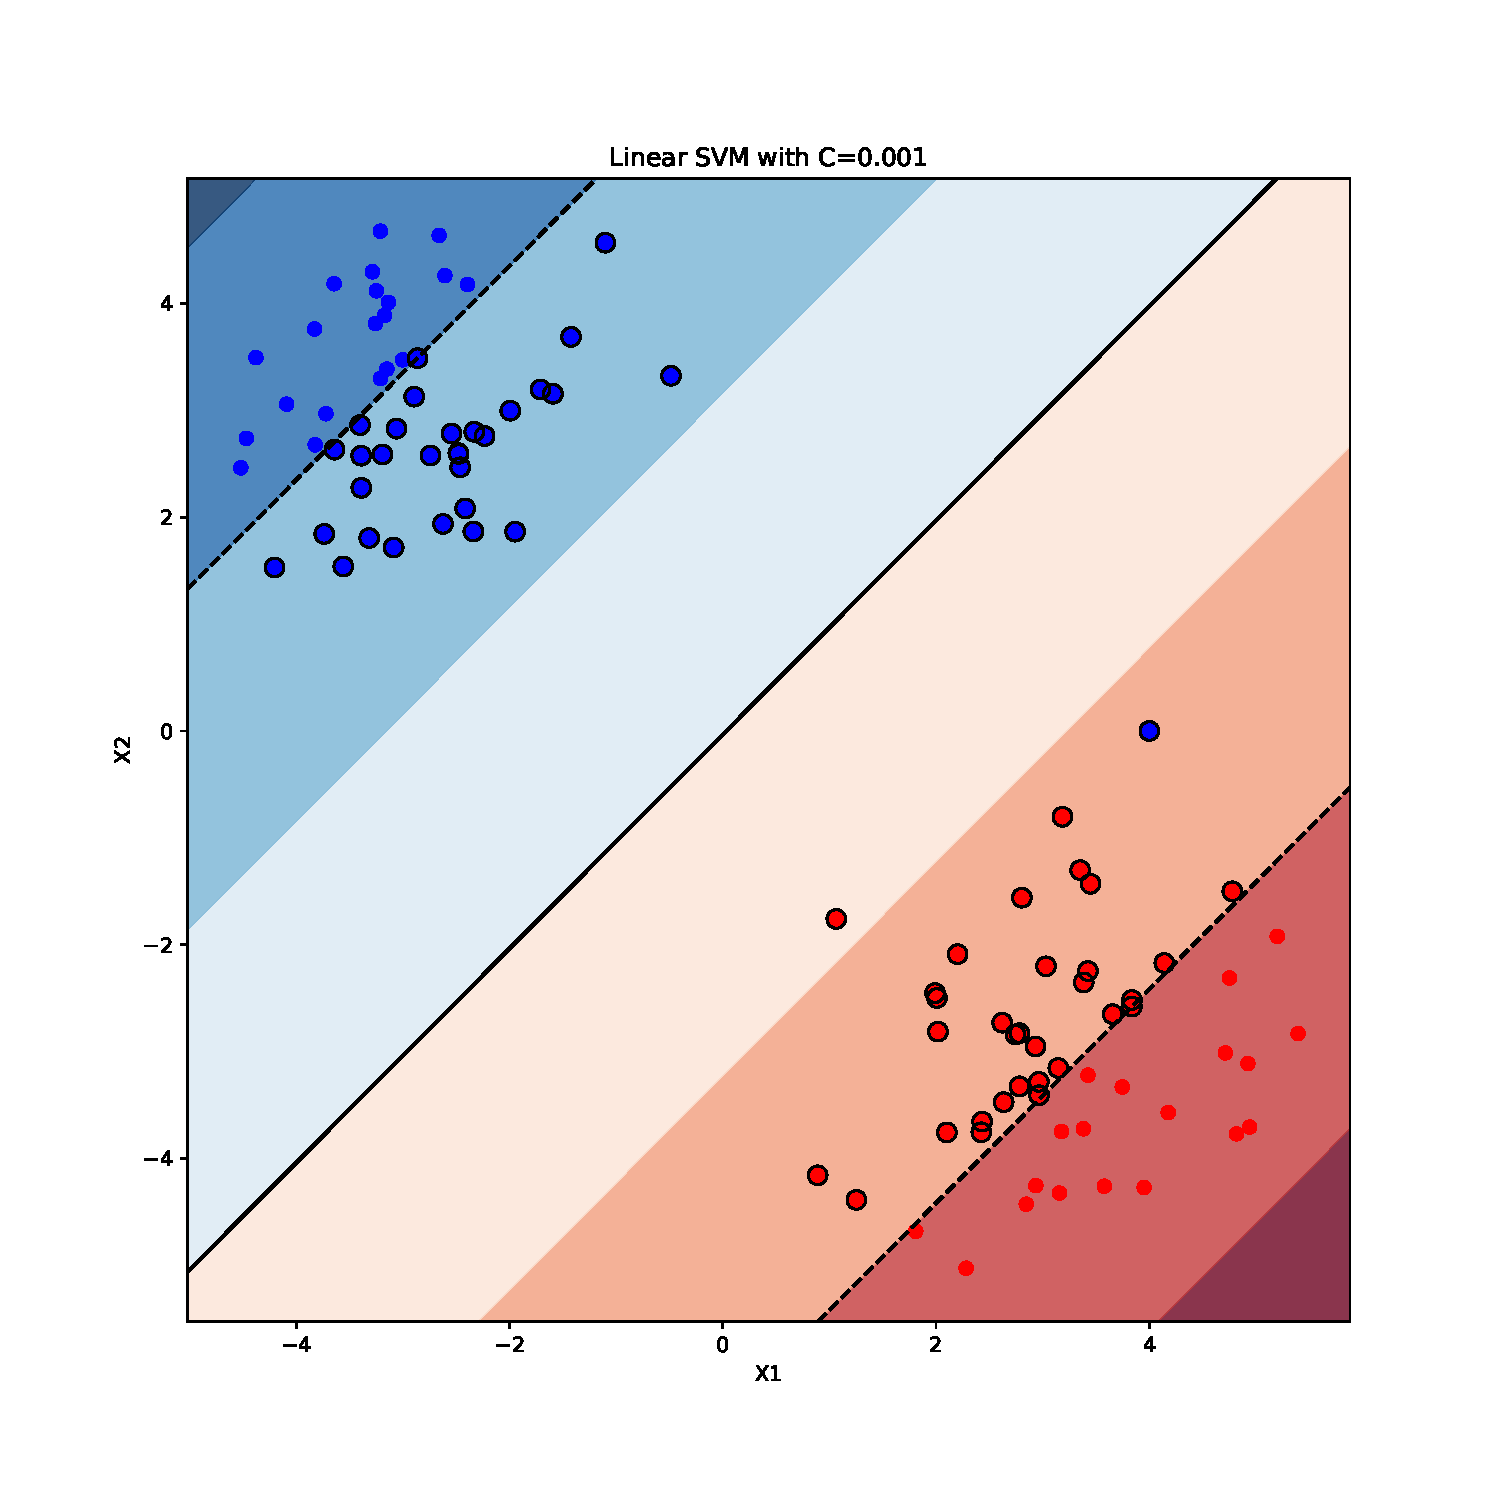
\includegraphics[width=\textwidth]{./Figures/1c_bound_C0001.pdf}
    \caption{$C=0,001$}
    \end{subfigure}
    \begin{subfigure}{0.6\textwidth}
    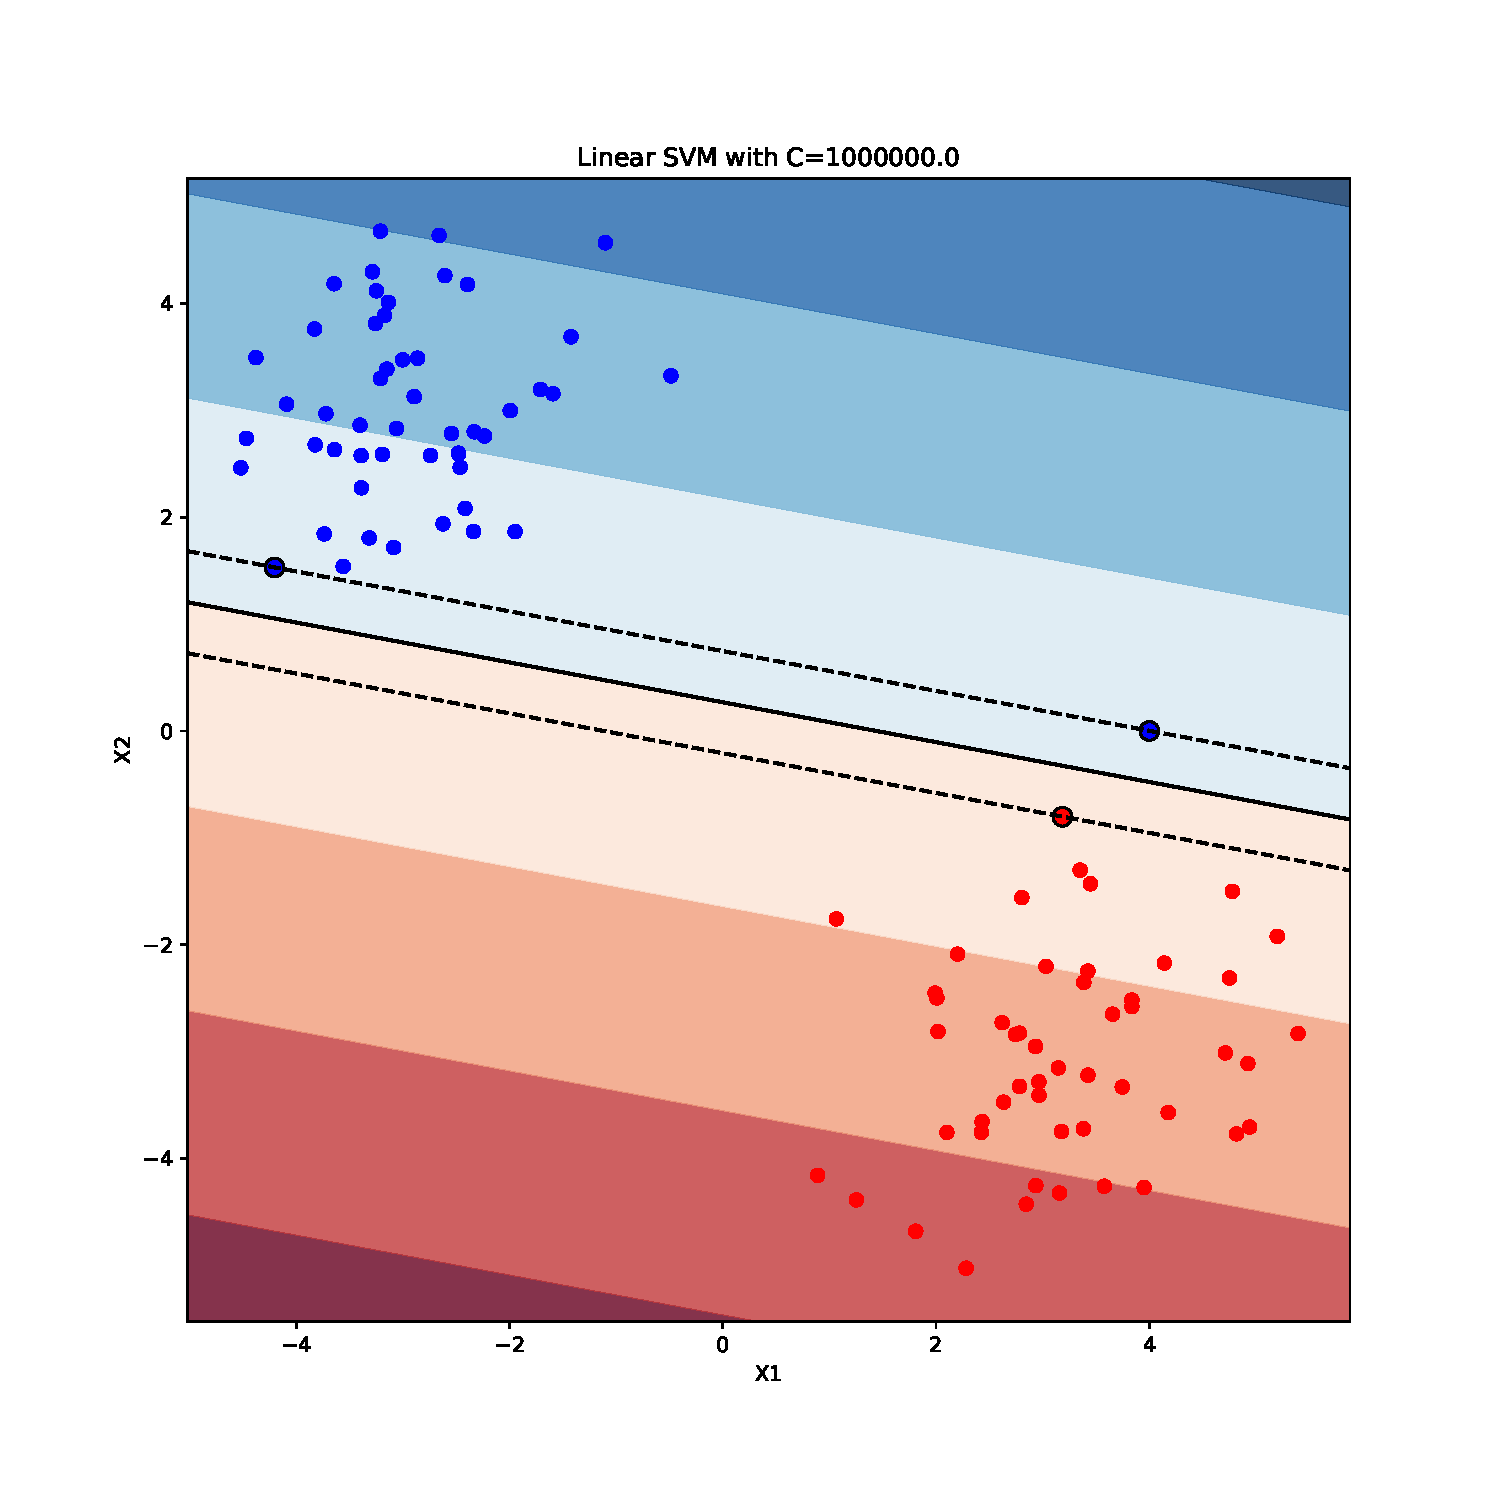
\includegraphics[width=\textwidth]{./Figures/1c_bound_C1e6.pdf}
    \caption{$C=1000000$}
    \end{subfigure}
    }
    \caption{SVM Classification using different C parameters}
    \label{SVM_Cs}
\end{figure}

\subsection{How and why changed the decision boundary when the new point was added?}

The margin is defined as the perpendicular distance between the decision boundary and the closest data point. Since the new added data point is located in the margin the algorithm adjusts its solution by choosing the option with the smallest generalization error. Apparently this solution includes more support vectors (datapoints within and on the margin boundary).

\subsection{The inverse regularization parameter $C$}

\begin{itemize}

	\item $C$ controls the penalization of data points within the margin. It is scaling data samples so that samples can be misclassified or lie within the margin boundary. This is helpful since not all problems can be clearly seperated.

	\item Figure \ref{SVM_Cs} is showing the classification using different values for $C$. The margin boundary gets larger with decreasing values for $C$. As a result the classification is showing more support vectors and also misclassifies the additional data point since these points are less penalized.
	    A very large value for C leads to the strict constraint that the margin borders are denoting the closest data point to the decision boundary. Therefore the margin boundary is very small.

\end{itemize}

\clearpage
\section{Nonlinear (kernel) SVM}

\begin{figure}[!ht]
\centering
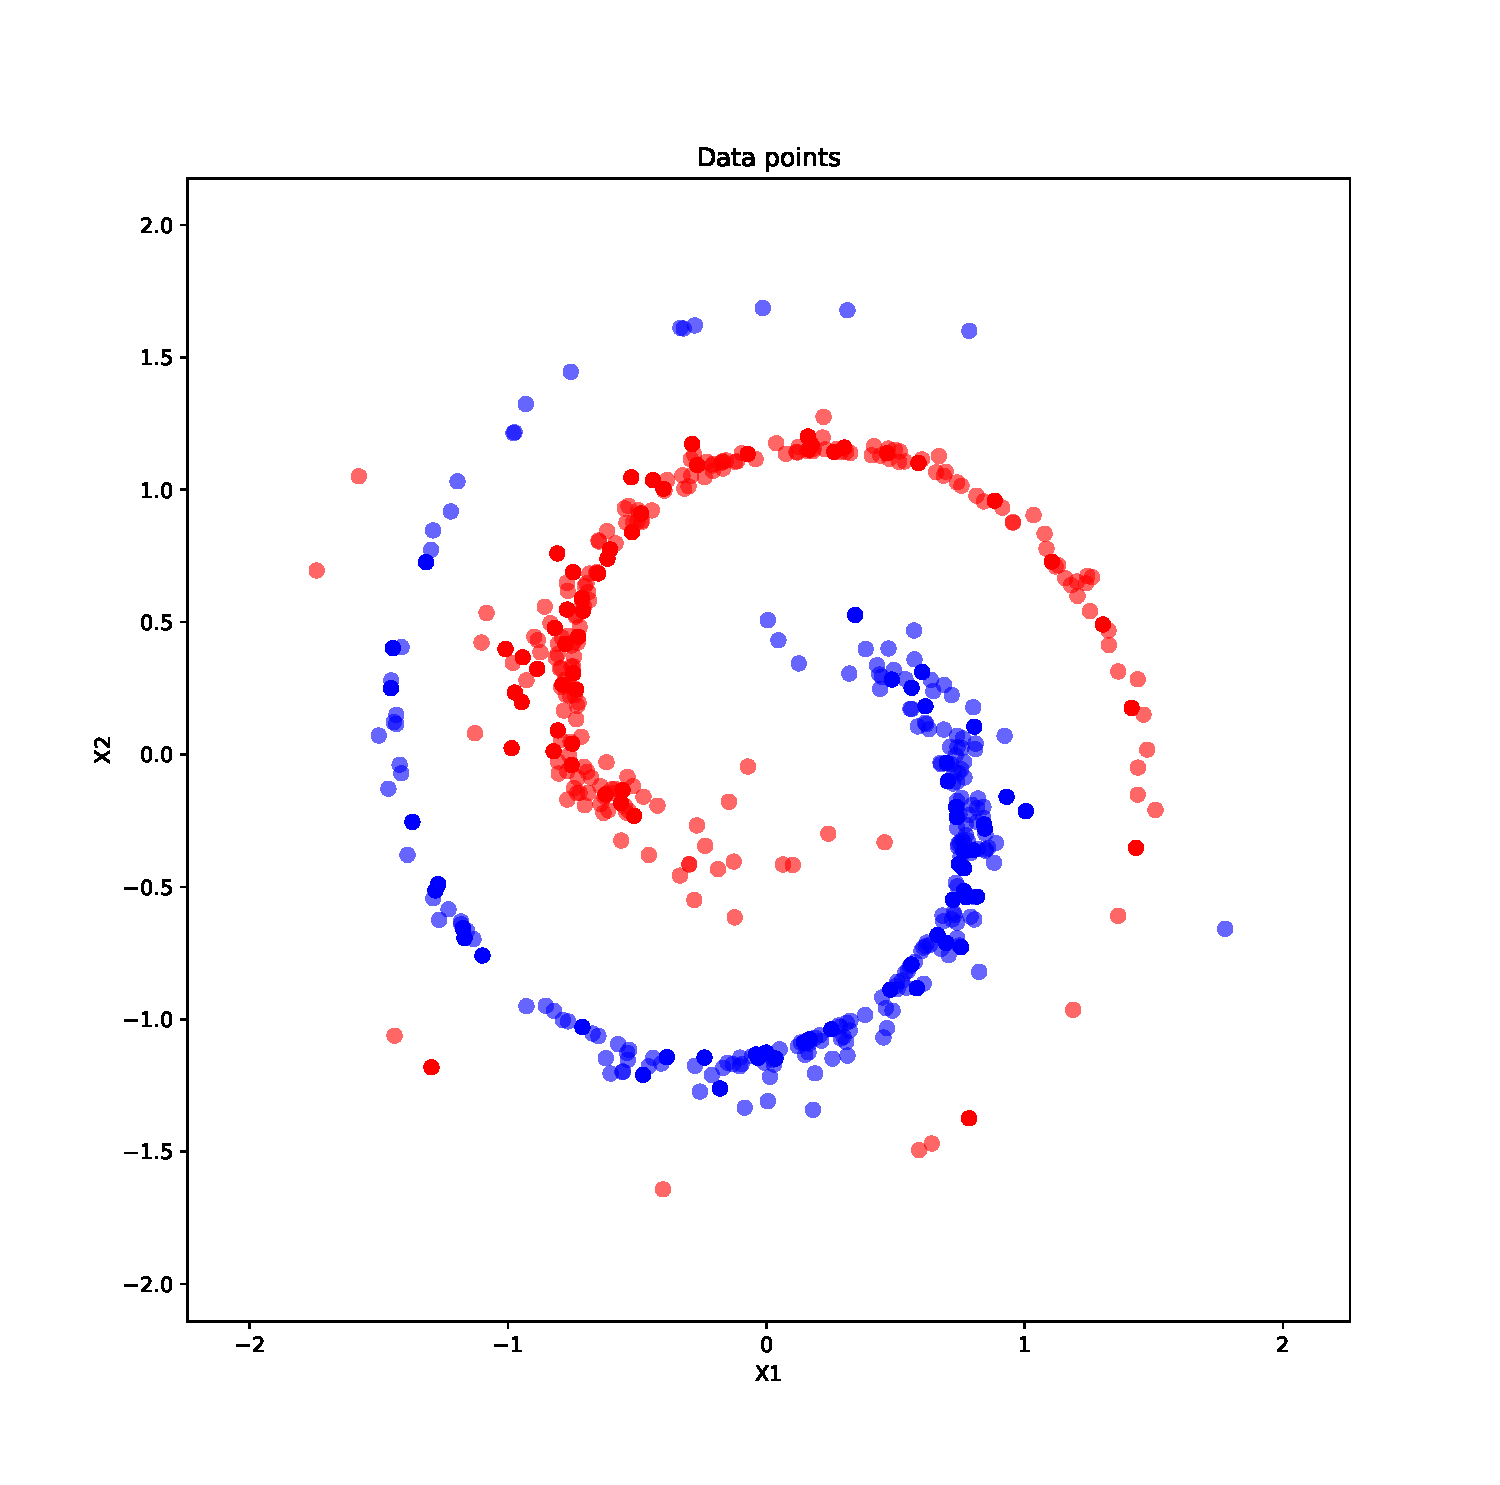
\includegraphics[width=0.55\textwidth]{./Figures/2_data.pdf}
\caption{Nonlinear binary classification problem.}
\label{2_data}
\end{figure}

\subsection{Linear kernel}

\begin{figure}[!ht]
\centering
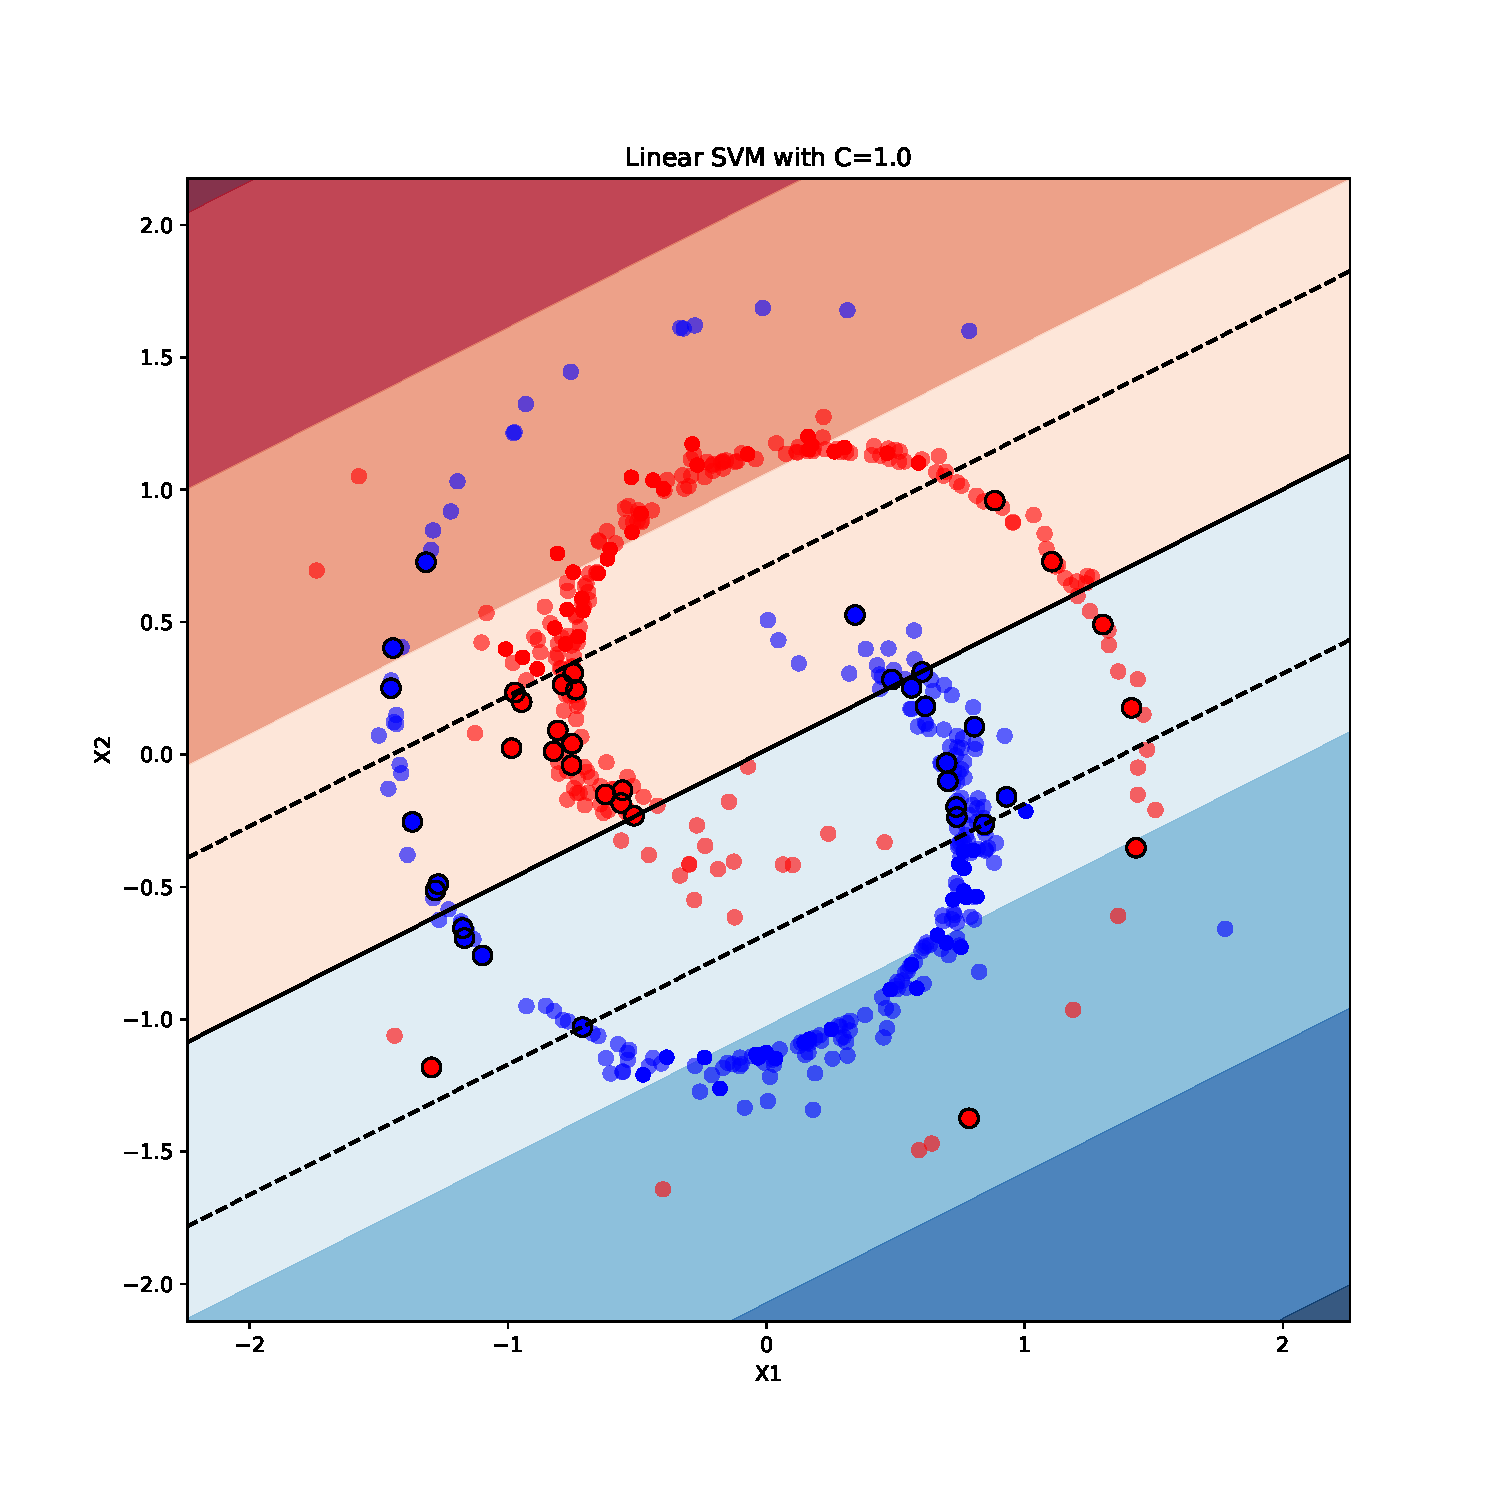
\includegraphics[width=0.65\textwidth]{./Figures/2a_bound_lin}
\caption{Decision boundary obtained by linear kernel.}
\label{2_bound_lin}
\end{figure}

\begin{table}[!ht]
\centering
\begin{tabular}{|c|} \hline
Test score \\ \hline
$81.25\%$\\ \hline
\end{tabular}
\caption{Test score obtained by linear kernel.}
\label{2_score_lin}
\end{table}

\subsection{Polynomial kernel}

\begin{figure}[!ht]
\centering
\begin{subfigure}{0.8\textwidth}
\centering
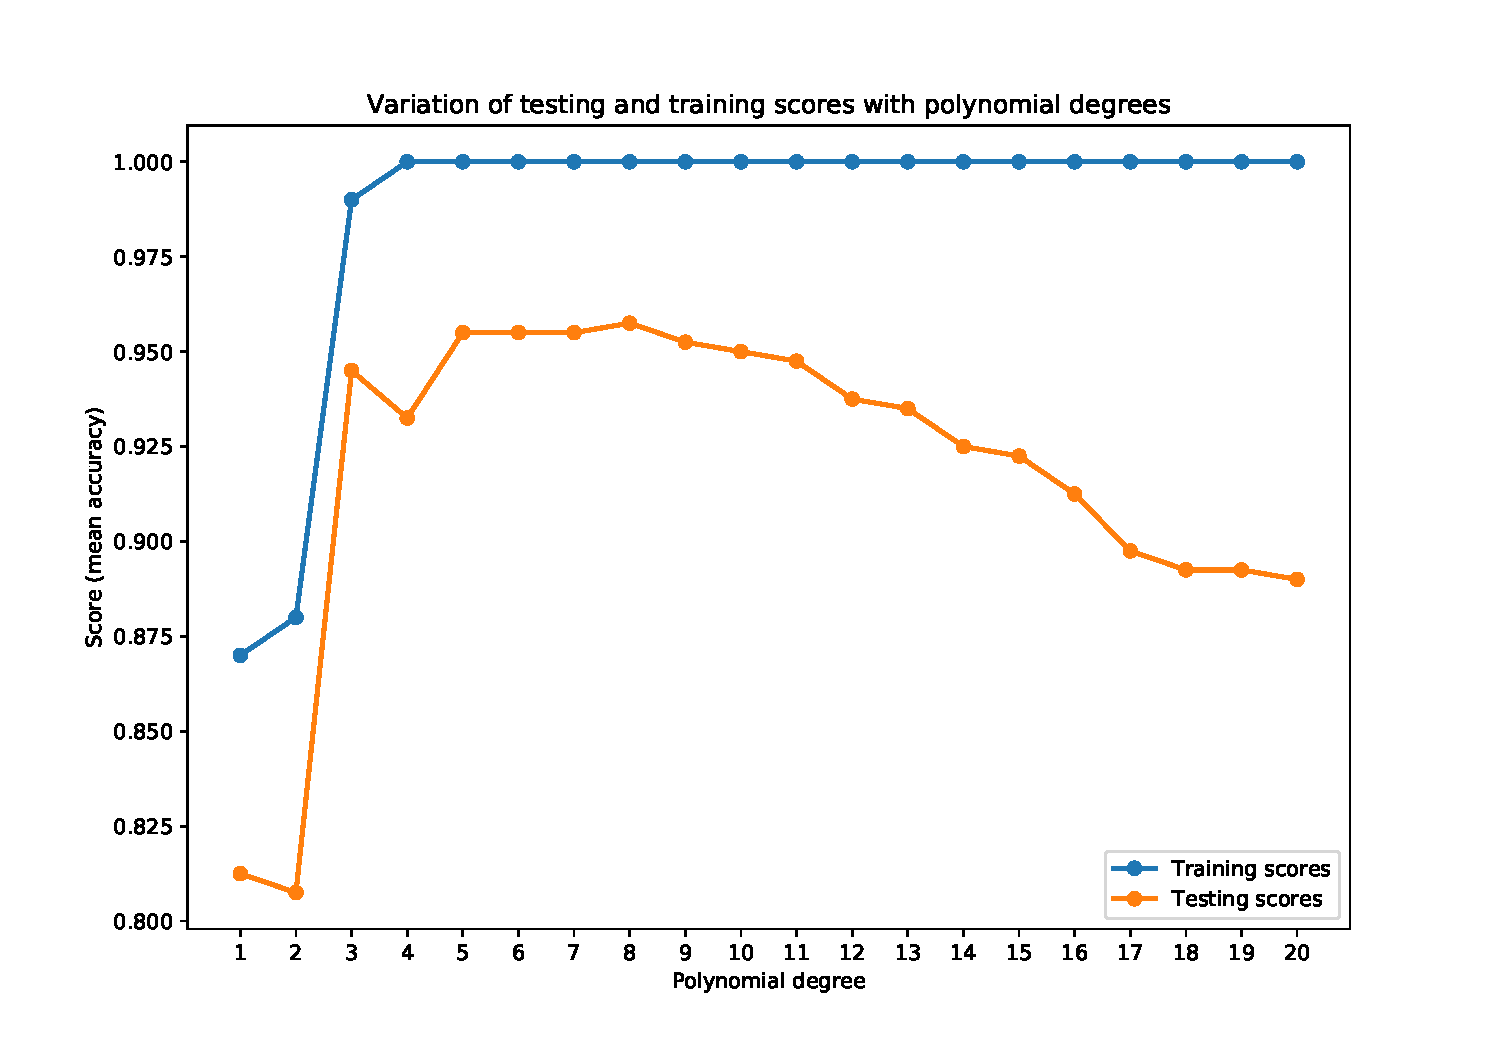
\includegraphics[width=\textwidth]{./Figures/2b_score_poly}
\caption{Score for varying polynomial degree.}
\label{2_score_poly}
\end{subfigure}

\begin{subfigure}{0.8\textwidth}
\centering
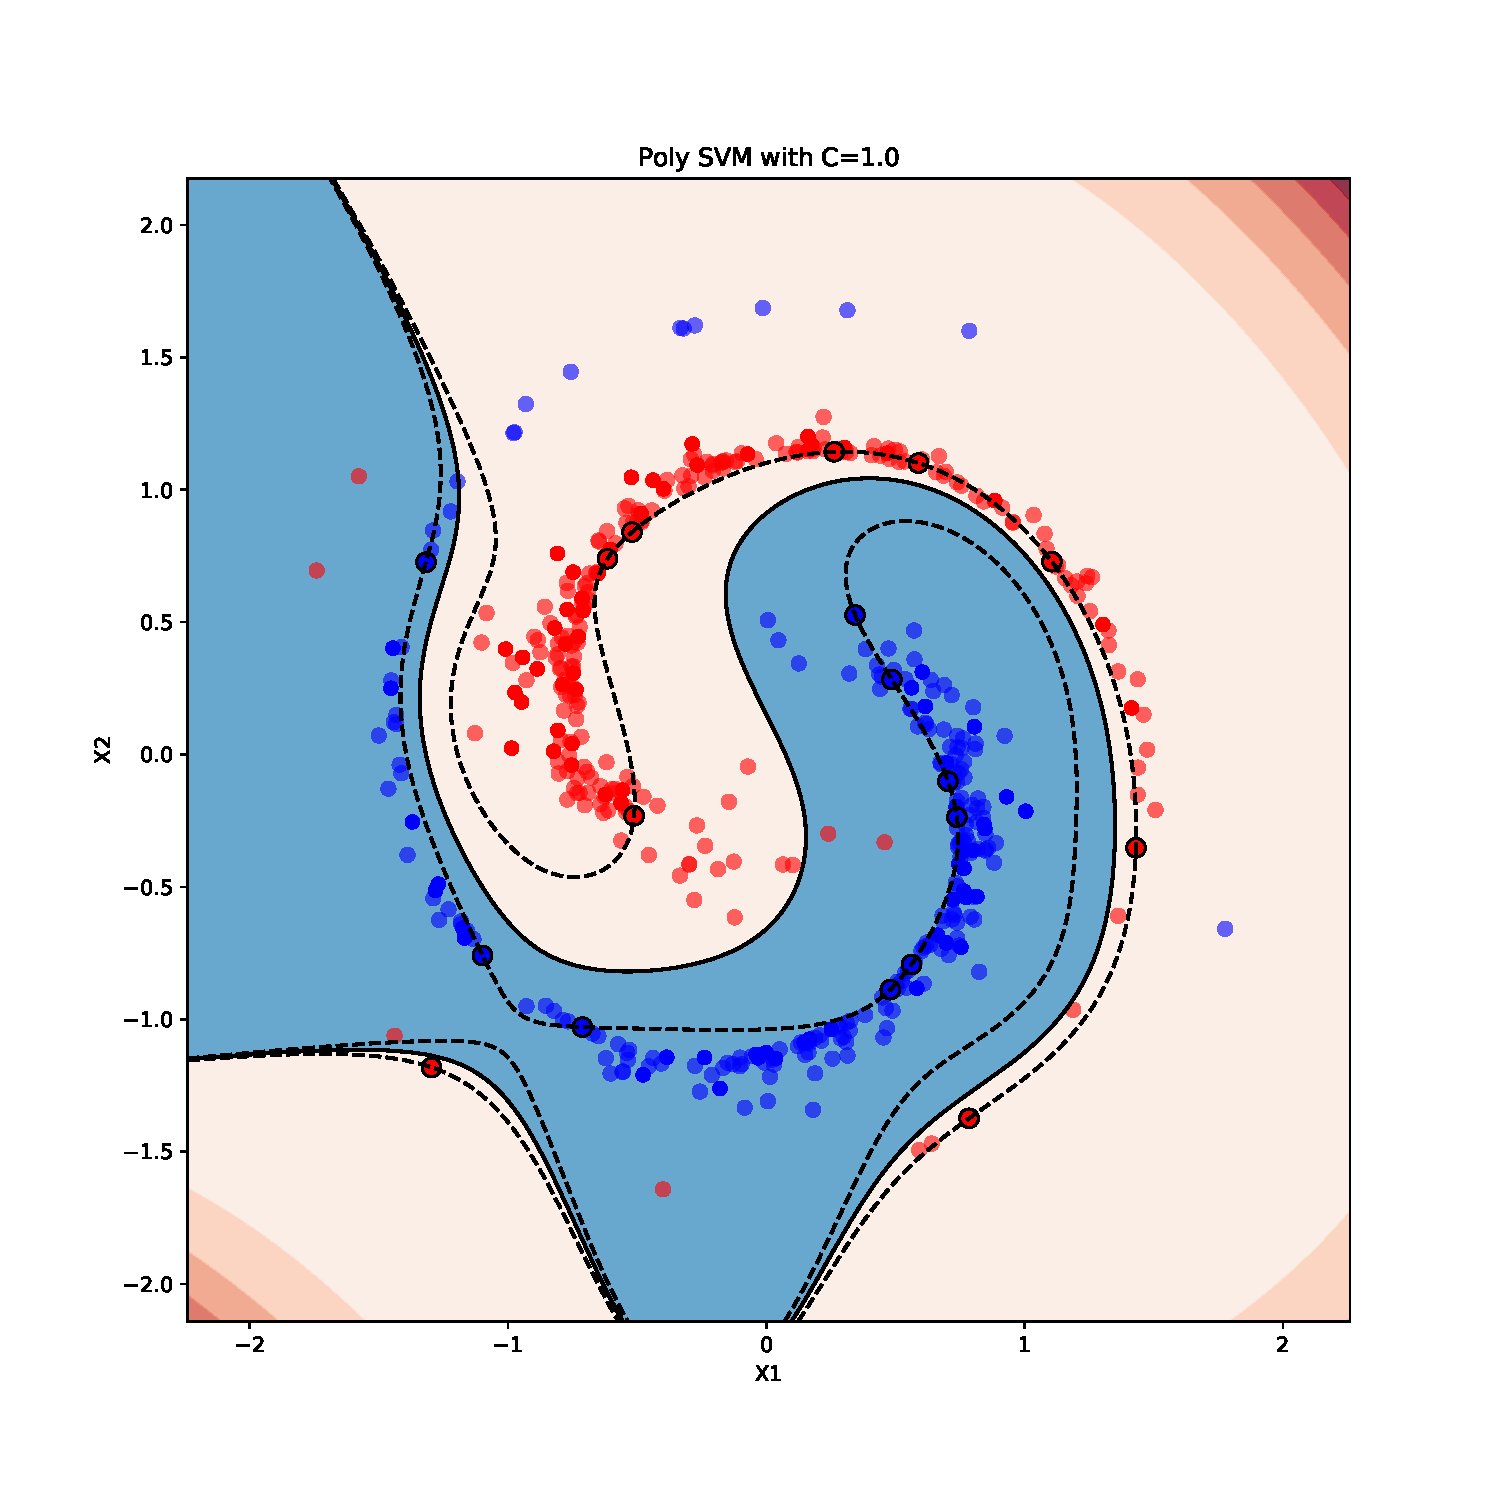
\includegraphics[width=\textwidth]{./Figures/2b_bound_poly}
\caption{Decision boundary for polynomial degree $8$.}
\label{2_bound_poly}
\end{subfigure}
\caption{Results obtained by polynomial kernel.}
\end{figure}

\begin{table}[!ht]
\centering
\begin{tabular}{|c|c|} \hline
Best degree & Test score \\ \hline
$8$ & $95.75\%$\\ \hline
\end{tabular}
\caption{Highest test score obtained by polynomial kernel.}
\label{2_best_poly}
\end{table}

\subsection{RBF kernel}

\begin{figure}[!ht]
\centering
\begin{subfigure}{0.8\textwidth}
\centering
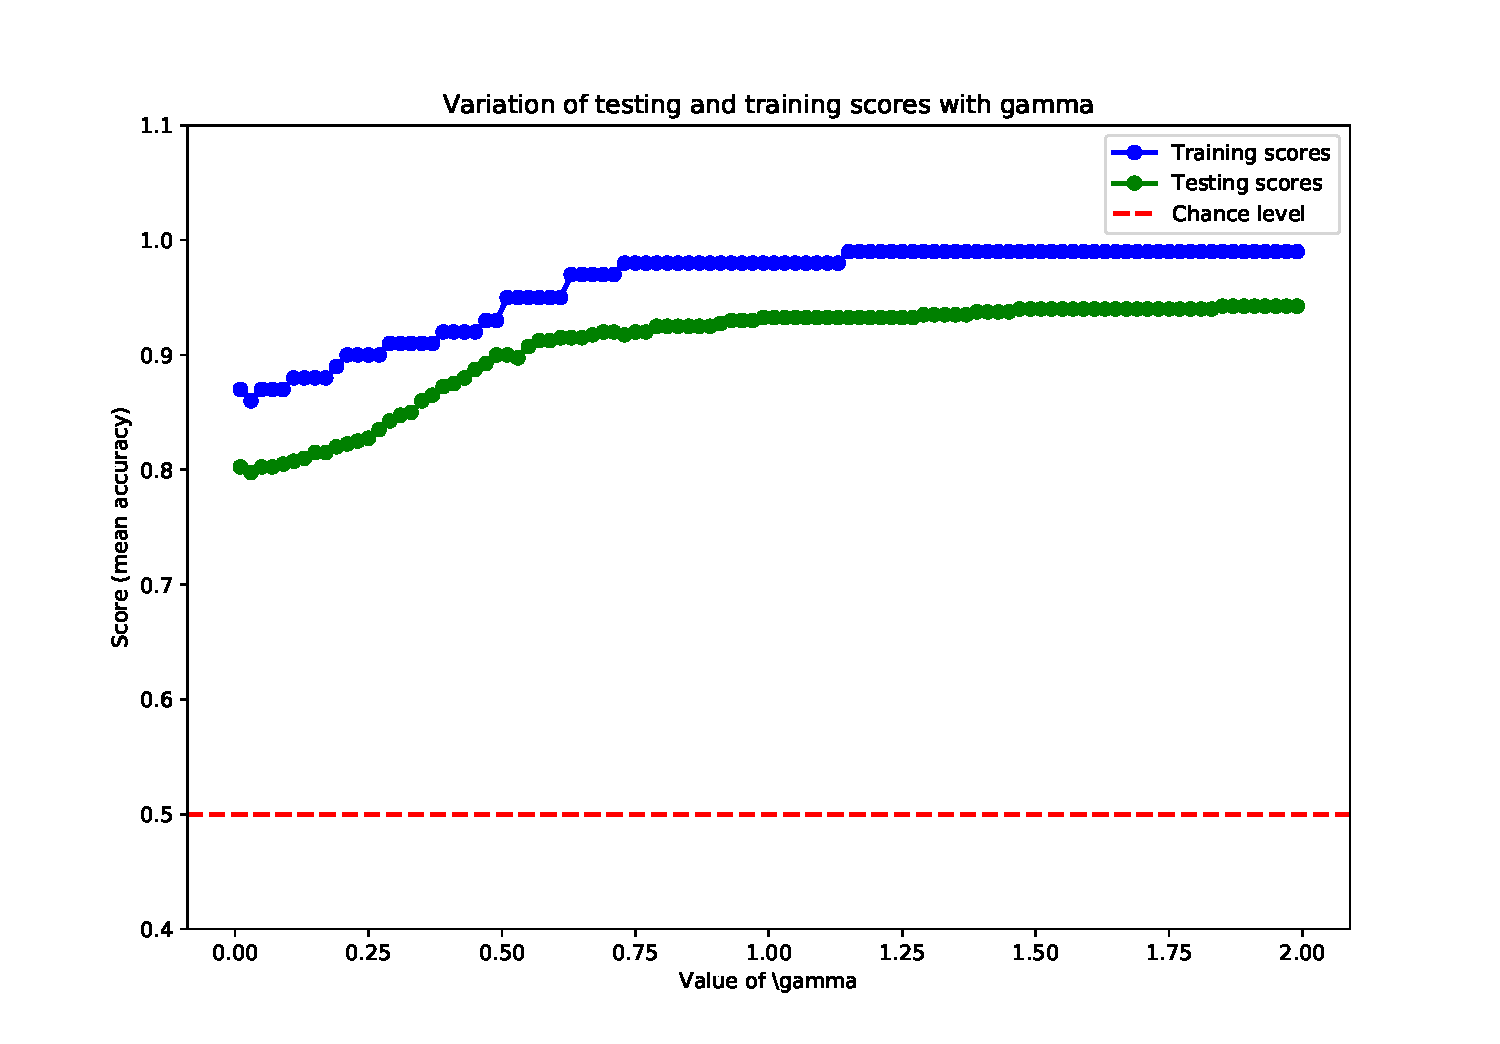
\includegraphics[width=\textwidth]{./Figures/2c_score_rbf}
\caption{Score for varying $\gamma$.}
\label{2_score_rbf}
\end{subfigure}

\begin{subfigure}{0.8\textwidth}
\centering
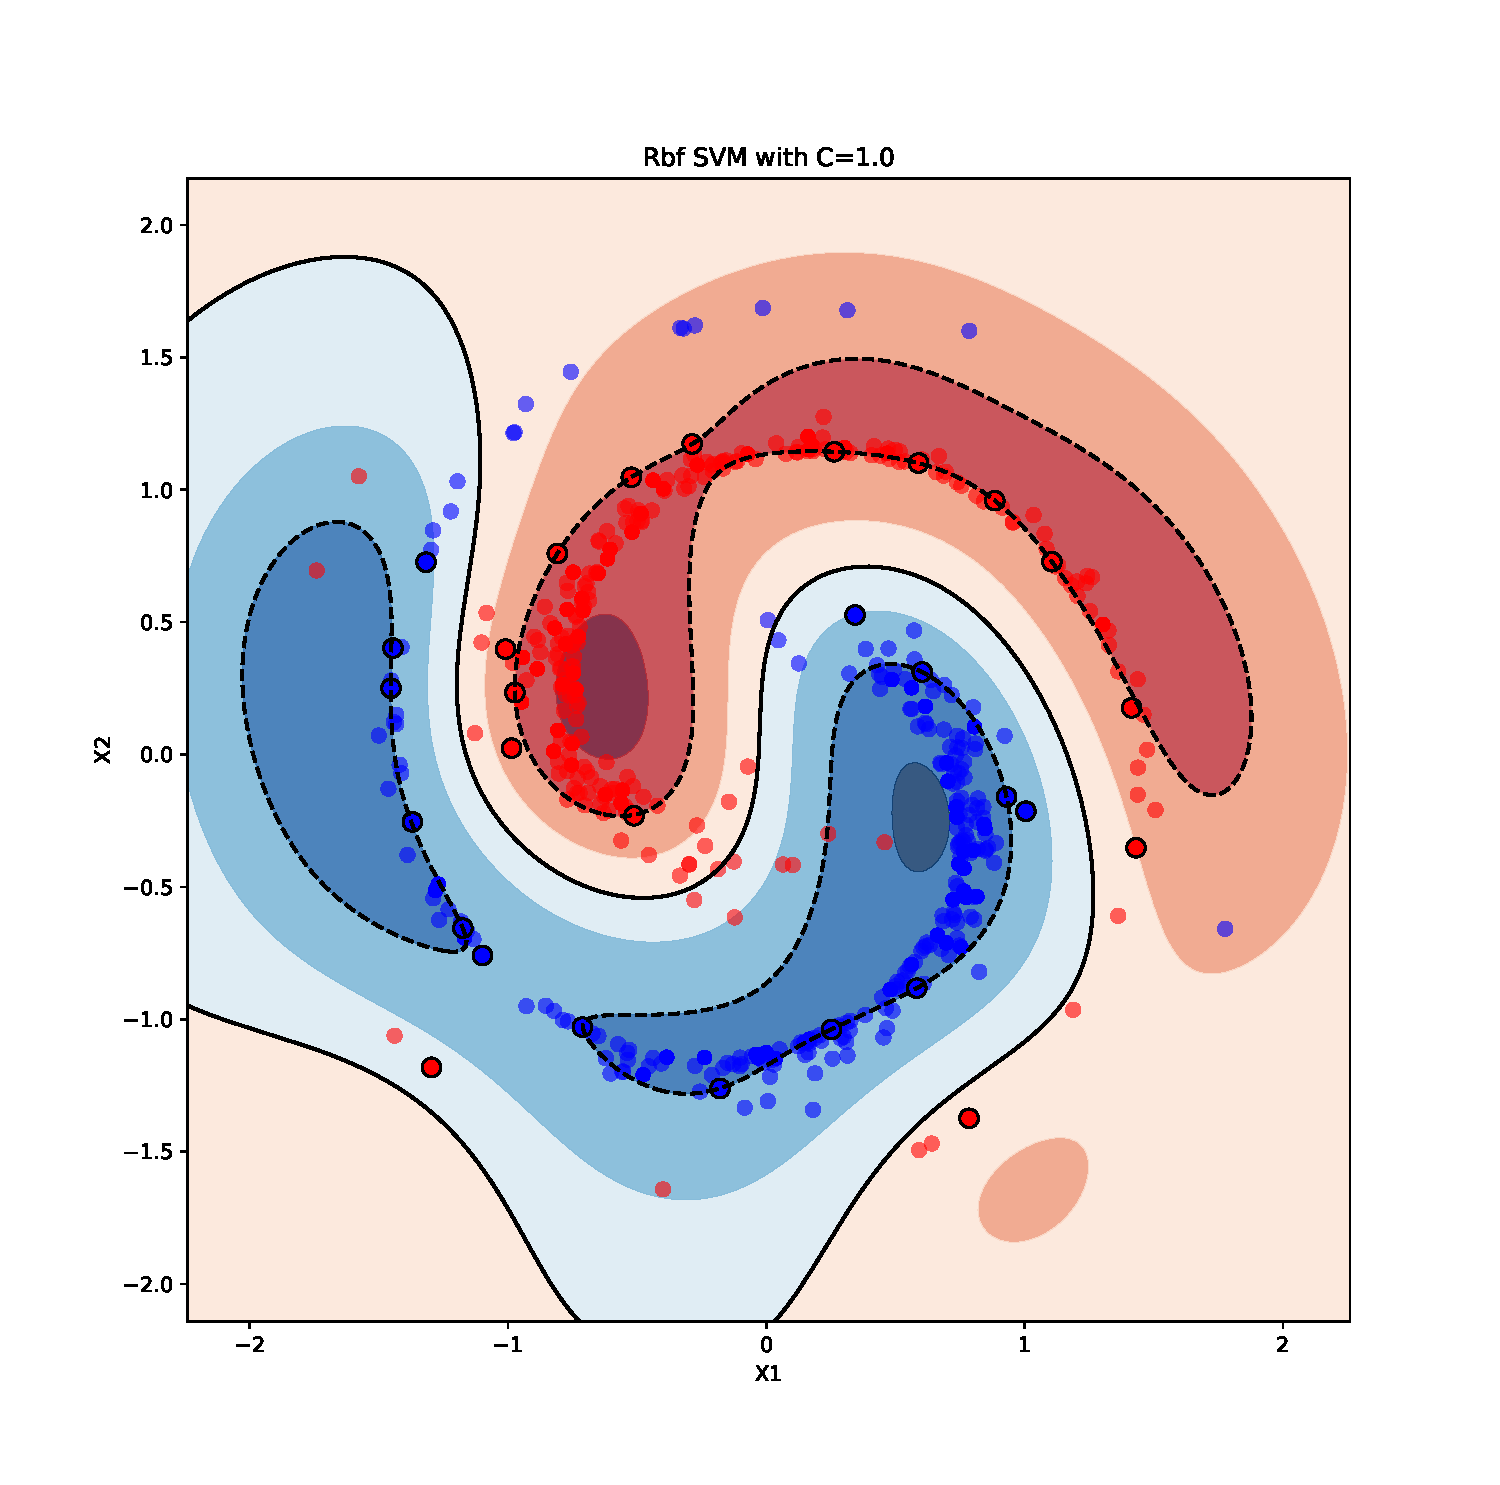
\includegraphics[width=\textwidth]{./Figures/2c_bound_rbf}
\caption{Decision boundary for $\gamma=1.85$.}
\label{2_bound_rbf}
\end{subfigure}
\caption{Results obtained by RBF kernel.}
\end{figure}

\begin{table}[!ht]
\centering
\begin{tabular}{|c|c|} \hline
Best $\gamma$ & Test score \\ \hline
$1.85$ & $94.25\%$\\ \hline
\end{tabular}
\caption{Highest test score obtained by RBF kernel.}
\label{2_best_rbf}
\end{table}

\subsection{Comparison of results obtained by each of the three kernels}

\begin{itemize}
\item While the linear kernel performs expectedly bad on nonlinearly separable data (s. figure \ref{2_bound_lin} and table \ref{2_score_lin}), testing scores obtained by polynomial kernels with degrees $3 \dots 13$ and RBF kernels with $\gamma \geq 1 $ are much higher (s. figures \ref{2_score_poly} and \ref{2_score_rbf}). A polynomial kernel with degree $8$ gives the best results (s. table \ref{2_best_poly}), in figure \ref{2_bound_poly} one can see that the support vectors that are used to produce the decision boundary exclusively lie on the margin boundaries (as opposed to the best RBF result in figure \ref{2_bound_rbf} and table \ref{2_best_rbf}).

\item Although the decision boundary obtained by the linear kernel is the most basic of the three, it takes the most support vectors, which are either misclassified or lie within the margin (s. figure \ref{2_bound_lin}). The polynomial kernel's decision boundary is more complex but at the same time relies on the least support vectors (exclusively on the margin borders, s. figure \ref{2_bound_poly}), because this approach fits the given data best. The most complex decision boundary (with insular patterns, s. figure \ref{2_bound_rbf}) is generated by the RBF kernel with a medium number of support vectors. Rather than only increasing with the complexity of the decision boundary, the number of needed support vectors also decreases the better the kernel fits the data.

\item The RBF kernel generalizes best, as both its training and testing scores continue to rise with increasing $\gamma$, without any overfitting (s. figure \ref{2_score_rbf}). Overfitting occurs when using the polynomial kernel with high degrees ($>>8$, s. figure \ref{2_score_poly})).

\end{itemize}

\clearpage
\section{Multiclass classification}

\subsection{}

\subsection{}

\subsection{}

\subsection{}

\clearpage
\section{SVM with Gradient Descent}

\subsection{Gradient Descent}

\begin{figure}[!ht]
\parbox[b]{\textwidth}{
\begin{subfigure}{0.6\textwidth}
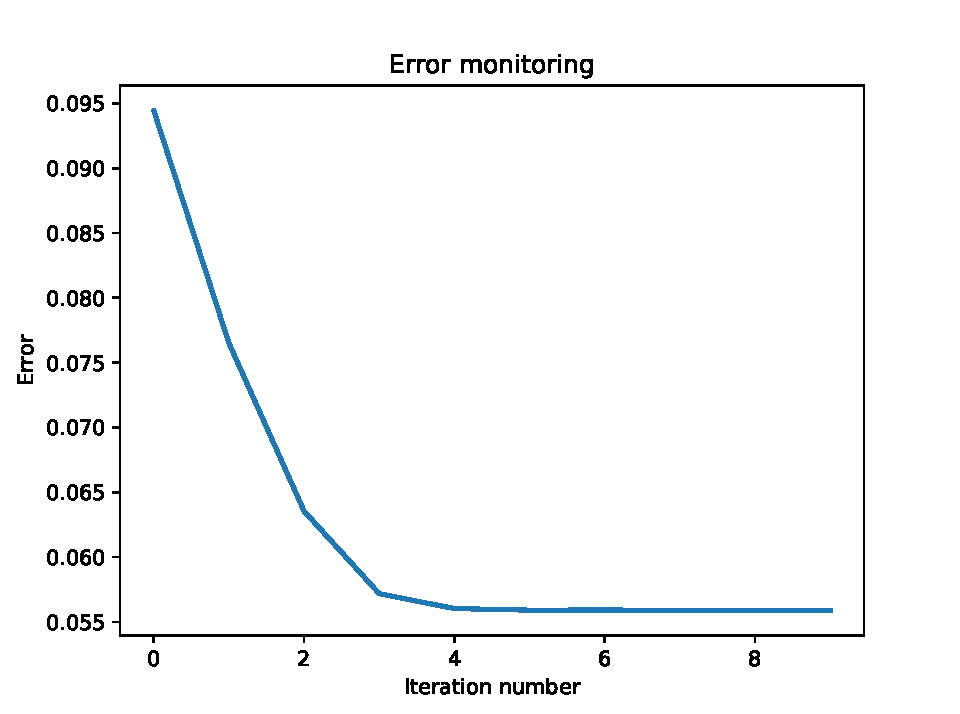
\includegraphics[width=\textwidth]{./Figures/4_error}
%\caption{Cost over iterations.}
%\label{4_cost}
\end{subfigure}
\begin{subfigure}{0.4\textwidth}
\begin{tabular}{|c|c|c|} \hline
$\mathbf{w}_{opt}$ & $b_{opt}$ & Final cost\\ \hline
$ \left[\begin{array}{r} -0.2195 \\ 0.2084 \end{array} \right]$ & $0.0025$ & $0.0569$\\ \hline
\end{tabular}
%\caption{Parameters and results.}
%\label{4_param_res}
\end{subfigure}
}
\caption{Results of GD.}
\label{4_GD}
\end{figure}

With the chosen number of iterations $10$ and step size $\eta=0.1$ the GD algorithm approximates the global minimum reasonably well and finds the optimal parameters $\mathbf{w}_{opt}$ and $b_{opt}$ (s. figure \ref{4_GD}).

\subsection{Results of classification}

\begin{figure}[!ht]
\centering
\begin{subfigure}{0.7\textwidth}
\centering
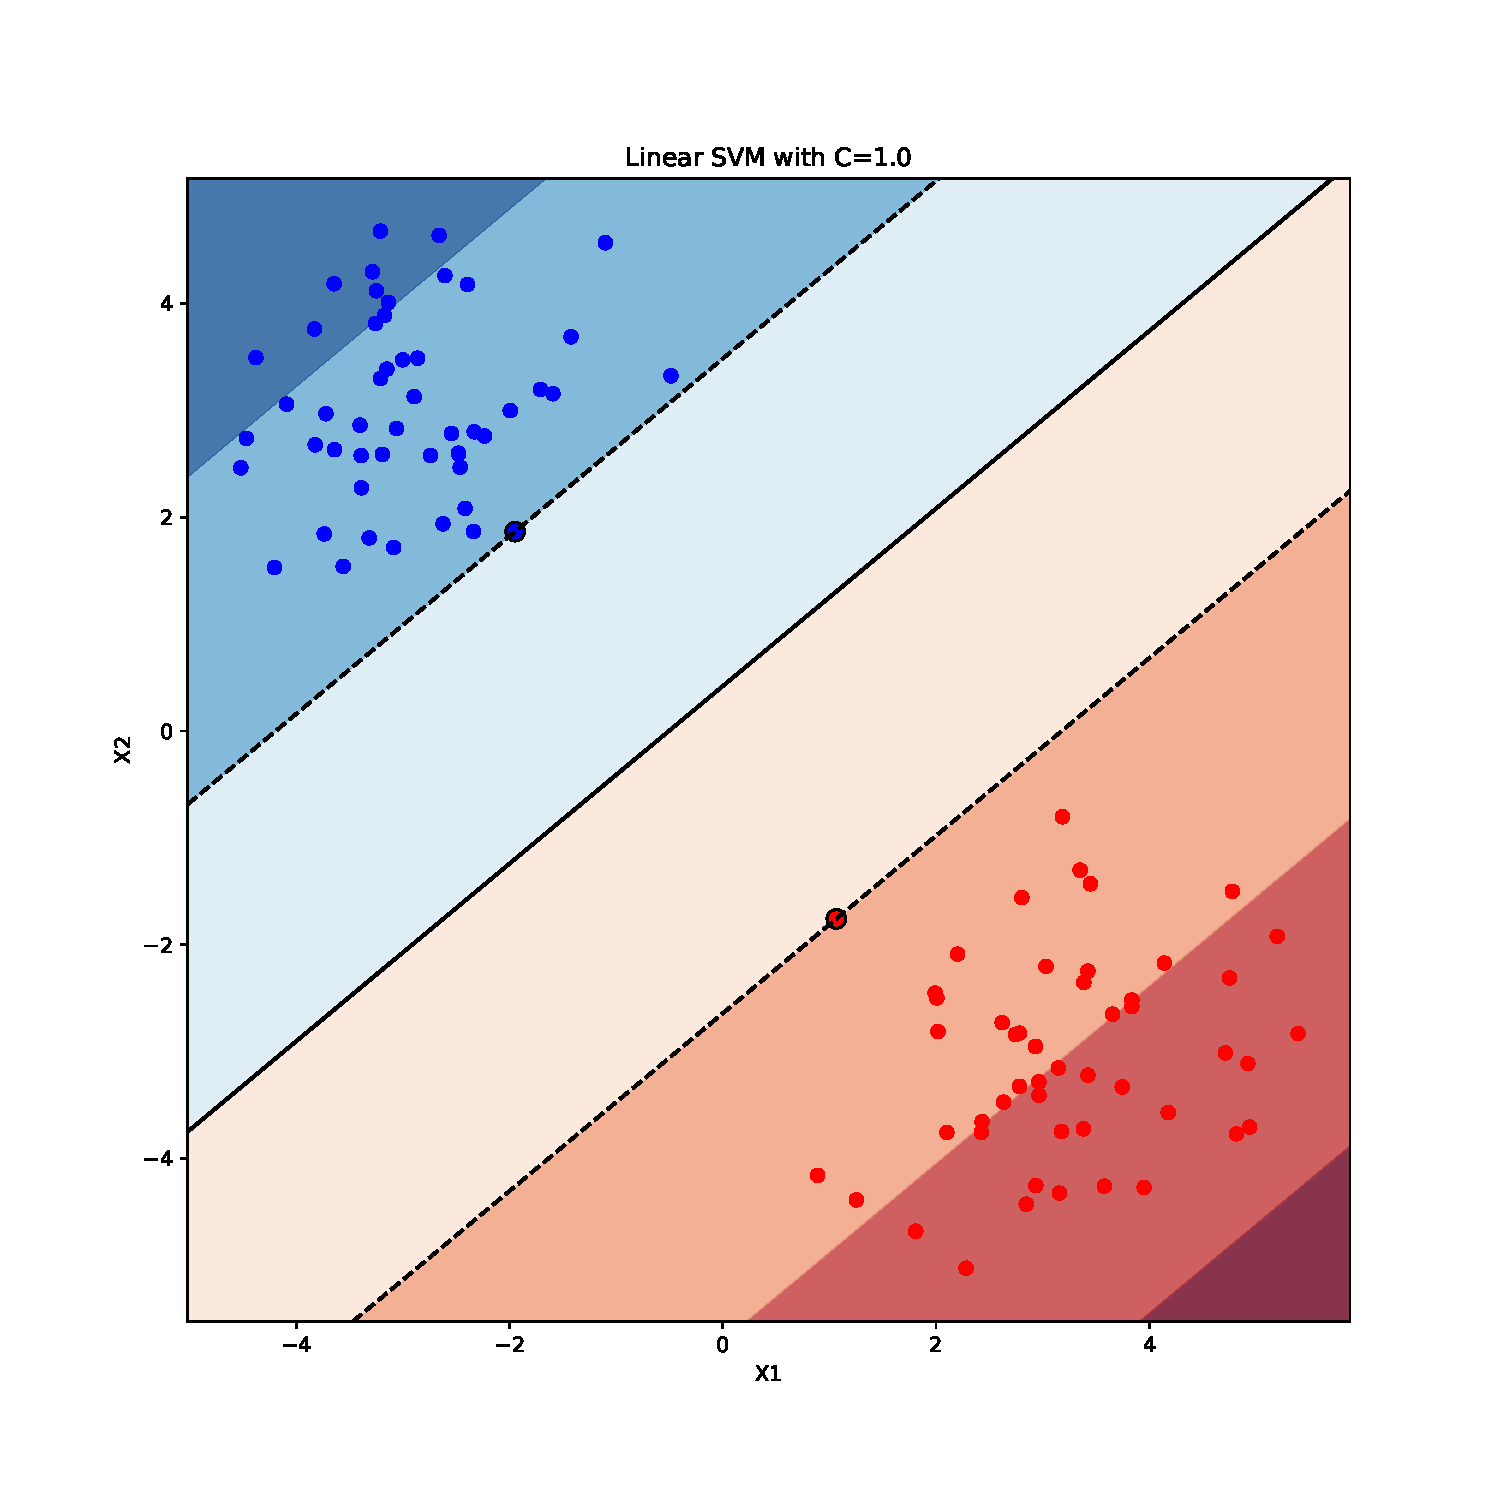
\includegraphics[width=\textwidth]{./Figures/1a_bound}
\caption{Task 1.}
\end{subfigure}
\begin{subfigure}{0.7\textwidth}
\centering
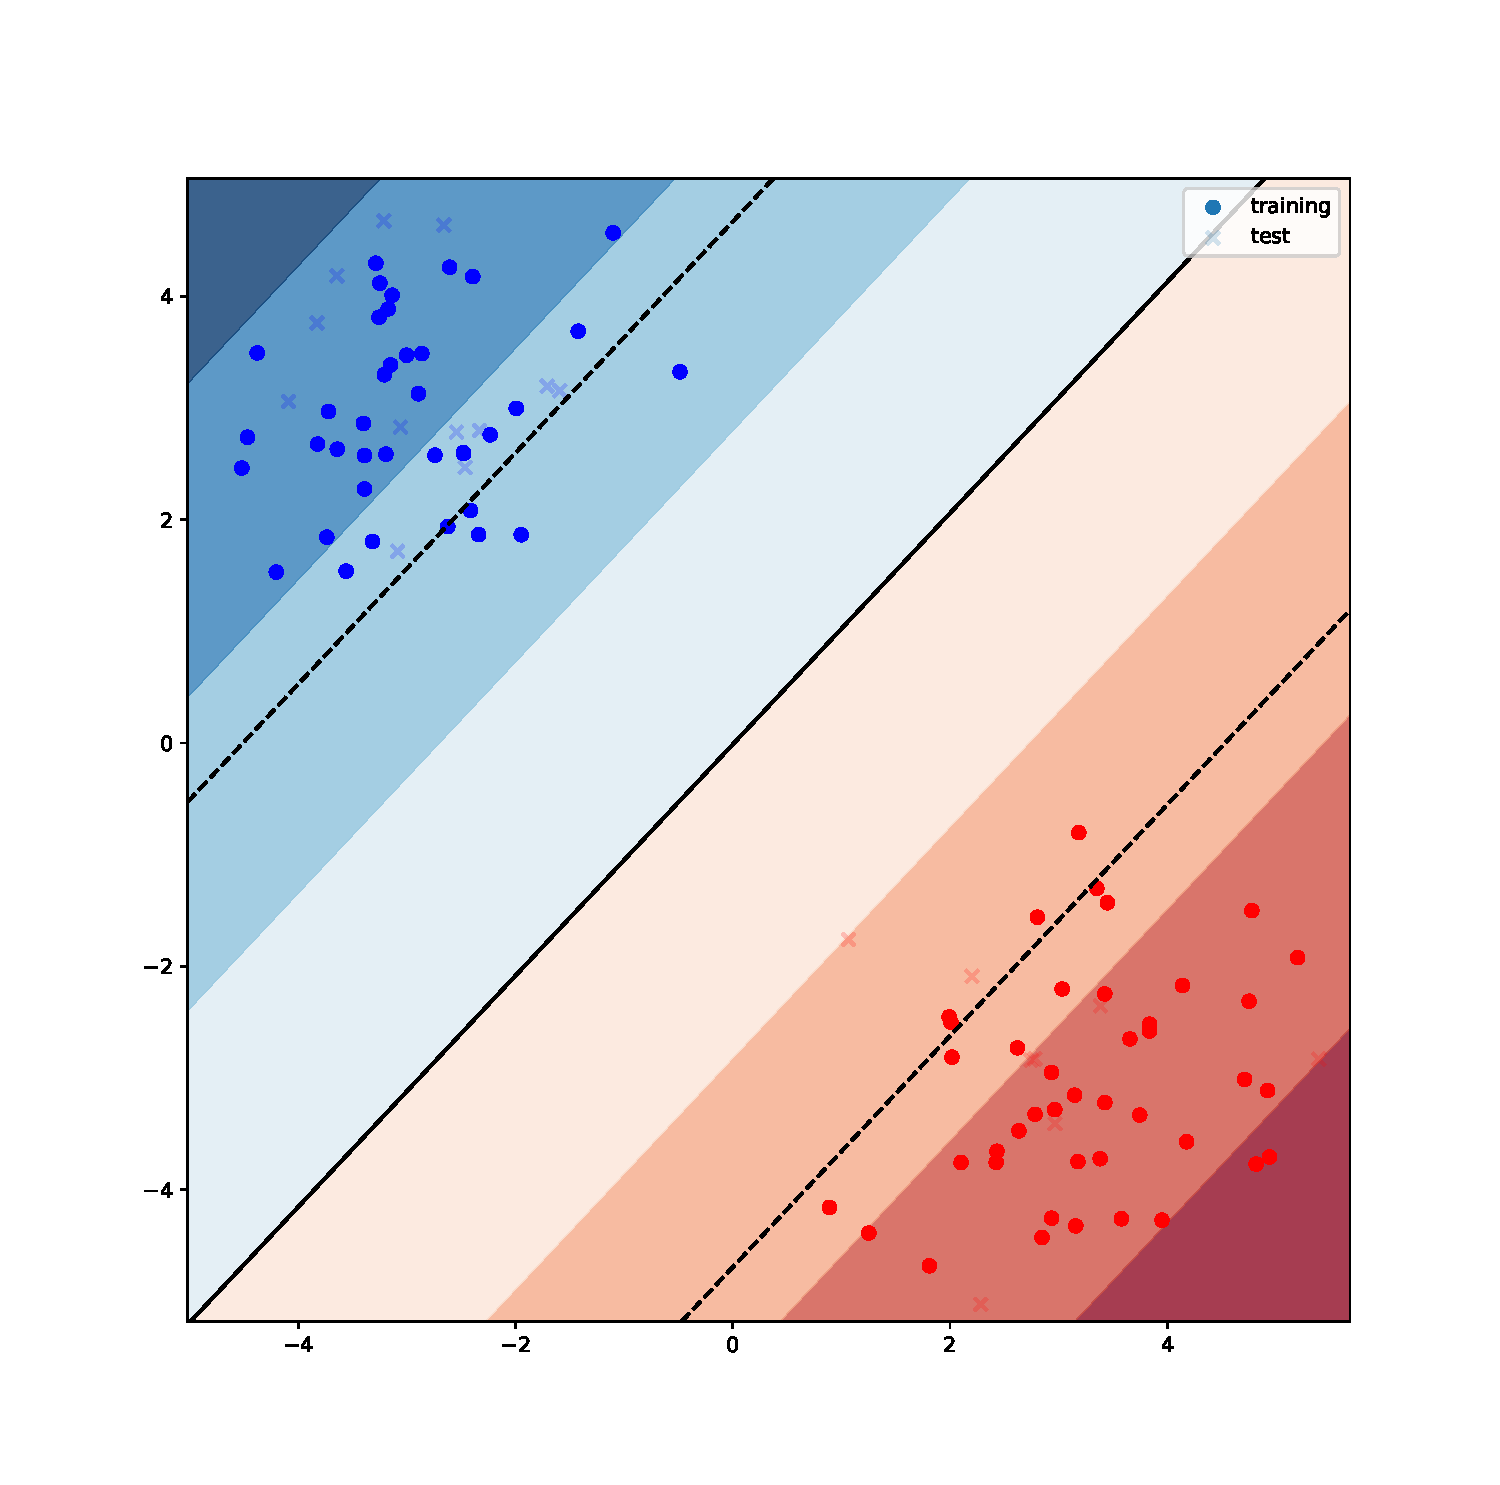
\includegraphics[width=\textwidth]{./Figures/4_bound}
\caption{Task 4.}
\label{4_4}
\end{subfigure}
\caption{Decision functions obtained by SVMs in tasks 1 and 4.}
\label{4_comp}
\end{figure}

Both SVM implementations from task 1 and 4 classify the dataset with an accuracy of $100\%$ (s. figure \ref{4_comp}). The first implementation's decision boundary relies on only two support vectors on the margin. The margin of the SVM implemented in task 4 is larger with samples lying within the margin as well. One reason for this could be the random separation of the data in training and testing sets. In figure \ref{4_4} the closest red point to the decision boundary is part of the testing set and can therefore not be used to generate the decision boundary.

\subsection{Drawbacks of Primal Formulation}

In Dual Formulation the dual coefficients $\alpha_i$ for all samples $i$ are known, i.e. one only needs to sum over the used support vectors to classify new samples. In Primal Formulation one needs to use the whole training set, leading to larger computational cost. Because the $max$-term of the Primal Formulation is non-smooth and therefore not differentiable at $y_i(\mathbf{w}^T\mathbf{x}_i+b) = 1$, subgradients with a conditional function $\mathbb{I}_i$ are needed. Then efficient GD solvers can be used.\\
Additionally - as opposed to Dual Formulation - the Kernel Trick can not be used, making the use of kernels more difficult.
\end{document}}